\documentclass[a4paper,10pt]{amsart}

\usepackage[protrusion=true,expansion=true]{microtype} 
\usepackage{fancyhdr}
\usepackage[utf8]{inputenc}
\usepackage{graphicx} 
\usepackage{wrapfig} 
\usepackage{enumitem}

\usepackage{mathpazo}
\usepackage[T1]{fontenc}
\usepackage{amsmath}
\usepackage{amssymb}
\usepackage{hyperref}
\usepackage{cleveref}
\usepackage[font=small,labelfont=bf,margin=\parindent,tableposition=top]{caption}
\usepackage{comment}
\usepackage{color}
\usepackage{mathtools}

%%%%%%%%% for quotation
\usepackage{microtype}
\usepackage{times}
\usepackage[english]{babel}
\usepackage{xcolor}
%%%%%%%%%%
% fancy quotes
%%%%%%%%%%
\definecolor{quotemark}{gray}{0.7}
\makeatletter
\def\fquote{%
    \@ifnextchar[{\fquote@i}{\fquote@i[]}%]
           }%
\def\fquote@i[#1]{%
    \def\tempa{#1}%
    \@ifnextchar[{\fquote@ii}{\fquote@ii[]}%]
                 }%
\def\fquote@ii[#1]{%
    \def\tempb{#1}%
    \@ifnextchar[{\fquote@iii}{\fquote@iii[]}%]
                      }%
\def\fquote@iii[#1]{%
    \def\tempc{#1}%
    \vspace{1em}%
    \noindent%
    \begin{list}{}{%
         \setlength{\leftmargin}{0.1\textwidth}%
         \setlength{\rightmargin}{0.1\textwidth}%
                  }%
         \item[]%
         \begin{picture}(0,0)%
         \put(-15,-5){\makebox(0,0){\scalebox{3}{\textcolor{quotemark}{``}}}}%
         \end{picture}%
         \begingroup\itshape}%
 %%%%%%%%%
 \def\endfquote{%
 \endgroup\par%
 \makebox[0pt][l]{%
 \hspace{0.8\textwidth}%
 \begin{picture}(0,0)(0,0)%
 \put(15,15){\makebox(0,0){%
 \scalebox{3}{\color{quotemark}''}}}%
 \end{picture}}%
 \ifx\tempa\empty%
 \else%
    \ifx\tempc\empty%
       \hfill\rule{100pt}{0.5pt}\\\mbox{}\hfill\tempa,\ \emph{\tempb}%
   \else%
       \hfill\rule{100pt}{0.5pt}\\\mbox{}\hfill\tempa,\ \emph{\tempb},\ \tempc%
   \fi\fi\par%
   \vspace{0.5em}%
 \end{list}%
 }%
 \makeatother

\newtheorem{example}{Example}[section]
\newtheorem{theorem}{Theorem}[section]
\newtheorem{proposition}{Proposition}[section]
\newtheorem{corollary}{Corollary}[section]
\newtheorem{definition}{Definition}[section]
\newtheorem{lemma}{Lemma}[section]
\newtheorem{remark}{Remark}[section]
\newtheorem{question}{Question}[section]
\newtheorem{conjecture}{Conjecture}[section]

\newcommand{\AAA}{\mathfrak A}
\newcommand{\BBB}{\mathcal B}
\newcommand{\CCC}{\mathcal C}
\newcommand{\HHH}{\mathcal H} %for Hilbert space
\newcommand{\LLL}{\mathcal L} % for lattice
\newcommand{\MMM}{\mathcal M}
\newcommand{\UUU}{\mathcal U}
\newcommand{\FFF}{\mathcal F}
\newcommand{\A}{\mathcal{A}}
\newcommand{\X}{\mathcal X}

\newcommand{\Lat}{\mathcal Lat}
\newcommand{\Alg}{\mathcal Alg}
\newcommand{\tensor}{\mathop{\bar \otimes}}
\newcommand{\tr}{\tau}
\newcommand{\C}{\mathbb C} %for complex number
\newcommand{\R}{\mathbb R}  %for real number
\newcommand{\Z}{\mathbb Z} %for integer
\newcommand{\N}{\mathbb N} % for nature number
\newcommand{\Q}{\mathbb Q} % for rational number

\providecommand{\sceil}[1]{\left \lceil #1 \right \rceil }
\providecommand{\sfloor}[1]{\left \lceil #1 \right \rceil }
\DeclarePairedDelimiter\ceil{\lceil}{\rceil}
\DeclarePairedDelimiter\floor{\lfloor}{\rfloor}
% self defined vars
\newcommand{\titleinfo}{Note on Sarnak Conjecture}
\newcommand{\authorinfo}{B. Fu, L. Ge, W. Yuan} 

\linespread{1.05}
\pagestyle{fancyplain}
\fancyhf{}
\fancyhf[HLE,HRO]{\titleinfo}
\fancyhf[HRE,HLO]{\authorinfo}
\fancyhf[FC]{\thepage}

\begin{document}

\title{\LARGE\textbf{\titleinfo}} 

\author{\large\textsc{\authorinfo}} 
\address{USTC}  
\email{}

\date{}

%\renewcommand{\abstractname}{Summary} 

\begin{abstract}
Enter abstract here
\end{abstract}

% Keywords
\subjclass[2010]{Primary 47L75; Secondary 15A30}
\keywords{M\"{o}bius function}

\thanks{}

\maketitle

\section{Introduction}
The M\"{o}bius function $\mu(n)$, $n = 1, 2, 3, \ldots$ is defined by
\begin{align*}
    \mu(n) = \begin{cases}
    1  \mbox{, if n=1}\\
    0  \mbox{, if n is not square free}\\
    (-1)^t \mbox{, if n is a product of t distinct primes}
  \end{cases} 
\end{align*}

Peter Sarnak give the disjointness conjecture concerning the M\"{o}bius 
function $\mu(n)$.
\begin{conjecture}[P. Sarnak]
    Let $(X, T)$ be a deterministic (i.e. the topological entropy h(T) = 0)
    topological dynamical system.
    \begin{align*}
        \lim_{n \rightarrow \infty}\frac{1}{n}\sum_{n}\mu(n)f(T^{n}x) = 0
    \end{align*}
    where $x \in X$ and $f \in C(X)$. 
\end{conjecture}

\section{Review on Entropy}
 \begin{fquote}
     [von Neumann said to Shannon]
     [Mathematical Theory of Entropy]
     [1981]
    You should call it entropy, for two reasons. In the 
    first place, your uncertainty function has been used in 
    statistical mechanics under that name, so it already has a name. 
    In the second place, and more important, no one knows what entropy
really is, so in a debate you will always have the advantage.
 \end{fquote}

Throughout this section ($X, \A, \mu$) denotes a measure space.

\subsection{Some ergodic results}

Let $T$ be a $\A$-measurable transformation from $X$ to $X$.
$\mu$ is $T$-invariant iff $\mu(T^{-1}B) = \mu(B)$ for every $B \in \A$.

\begin{definition}
   Let $T : X  \rightarrow X$ be a transformation. The periodic entropy
   of $T$ is 
   \begin{align*}
       p(T) = \lim_{m \rightarrow \infty} sum \frac{1}{m}
       log(\#\{x \in X : T^{m}(x)=x \}).
   \end{align*}
\end{definition}

\begin{remark}
   The periodic entropy measures the complexity of $T$ from the 
   point of view of the periodic points. For example, let 
   $T : z \rightarrow z^m$ from $S^1$ to $S^1$, 
   $p(T) = log|m| >0$.
\end{remark}

\begin{theorem}[$Poinca\acute{r}e$'s recurrence theorem]
   Let $T : X \rightarrow X$ be a measurable transformation and 
   let $\mu$ be a finite $T$-invariant measure in $X$. If $A \subset X$
   is measurable, then the set
   \begin{align*}
    B = \{ x \in A: T^n (x) \in A 
    \mbox{, for infinitely many integers n} \in \N \} 
   \end{align*}
   has measure $\mu(B) = \mu(A)$.
\end{theorem}

\begin{definition}
   Given a transformation $T: X \rightarrow X$, we say that 
   a function $\varphi$ is $T$-invariant if $\varphi(T(x)) = T(x)$ for 
   every $x \in X$. $\varphi$ is $T$-invariant almost everywhere
   if there is a $T$-invariant subset $B \subset X$, i.e. 
   $T^{-1}B = B$, with $\mu(X \setminus B) = 0$ and $\varphi|_{B}$ is
   $T$-invariant.
\end{definition}

\begin{theorem}[Birkhoff's ergodic theorem]
   Let $T : X \rightarrow X$ be a measurable transformation
   and let $\mu$ be a finite $T$-invariant measure in $X$. If
   $\varphi \in L^{1}(X, d\mu)$, then the limit
   \begin{align*}
       \varphi_{T} = \lim_{n \rightarrow \infty}\frac{1}{n}
       \sum_{k = 0}^{n} \varphi(T^k (x))
   \end{align*}
   \begin{itemize}
       \item $\varphi_{T}$ is T-invariant almost everywhere.
       \item $\varphi_{T} \in L^{1}(X, d\mu)$ and 
           $\int_{X}\varphi_{T} d\mu = \int_{X} \varphi d\mu$.
   \end{itemize}
\end{theorem}

\subsection{Metric(measure-theoretical) Entropy}
In this subsection we assume that $\mu(X) = 1$.
Let
\begin{align*}
    \psi(x) = \begin{cases}
    xlogx  \mbox{, if x $\neq$ 0}\\
    0  \mbox{, if x=0.}\\
  \end{cases} 
\end{align*}

\begin{definition}
   Let $\xi \subset \A$. If
   \begin{enumerate}
       \item $\mu(\cup_{C \in \xi} C) = 1$,
       \item $\mu(C \cap D) = 0$ for any distinct $C$, $D$ in $\xi$,
   \end{enumerate}
   then $\xi$ is a measurable partition of $(X, \A, \mu)$.
\end{definition}

\begin{definition}[Entropy of a measurable partition]
   Let $\xi$ be a measurable partition of $X$ w.r.t $\mu$. The
   entropy of $\xi$ is given by
   \begin{align*}
       H_{\mu}(\xi) = -\sum_{C \in \xi}\mu(C)log\mu(C)
       = -\sum_{C \in \xi}\psi(\mu(C)).
   \end{align*}
\end{definition}

\begin{definition}
   Given two measurable partition $\xi$, $\eta$ of $X$, we 
   define a new measurable partition
   \begin{align*}
       \xi \bigvee \eta = \{C \cap D: C\in \xi, D \in \eta \}. 
   \end{align*}
\end{definition}

\begin{definition}
   Let $T: X \rightarrow X$ be a measurable transformation preserving 
   the probability measure $\mu$ and $\xi$ a measurable partition of $X$.
   The metric entropy of $T$ with respect to $\mu$ and $\xi$ is 
   \begin{align*}
       h_{\mu}(T, \xi) = \lim_{n \rightarrow \infty} \frac{1}{n}H_{\mu}(\xi_n)
       = \inf_{n \in \N} H_{\mu}(\xi_n),
   \end{align*}
   where $\xi_n = \bigvee_{k=0}^{n-1} T^{-k}\xi$.
   The metric entropy of $T$ with respect to $\mu$ is 
   \begin{align*}
       h_{\mu}(T) = sup\{h_{\mu}(T, \xi): \xi 
       \mbox{is  a measurable partition of X} \}. 
   \end{align*}
\end{definition}

\begin{lemma}
   Let $\xi$ and $\eta$ be measurable partitions of $X$. If $\eta$ is 
   a refinement of $\xi$, i.e., each element of $\xi$ is a union of 
   elements of $\eta$, then $H_{\mu}(\xi) \leq H_{\mu}(\eta)$.
\end{lemma}

\begin{theorem}
   Let $T: X \rightarrow X$ be a measurable transformation preserving 
   the probability measure $\mu$. If $(\xi_{n})_{n \in \N}$ is a sequence
   of  measurable partitions of $X$ with $\bigvee^{\infty}_{n = 1}\A(\xi_n)$
   ($\A(\xi)$ is the $\sigma$-algebra generated by $\xi$) such that 
   $\xi_{n+1}$ is a refinement of $\xi_{n}$ for each $n \in N$, then
   \begin{align*}
       h_{\mu}(T) = \lim_{n \rightarrow \infty}h_{\mu}(T, \xi_{n})
       = sup_{n \in \N} h_{\mu}(T, \xi_n).
   \end{align*}
\end{theorem}
 
Specially, if $\bigvee_{k=0}^{\infty} \A(T^{-k}\xi) = \A$ or 
$\bigvee_{k=-\infty}^{\infty} \A(T^{-k}\xi) = \A$, 
then we have the following.

\begin{corollary}
    Let $T: X \rightarrow X$ be a measurable transformation preserving 
    the probability measure $\mu$. If $\bigvee_{k=0}^{\infty} \A(T^{-k}\xi) = \A$ or 
    $\bigvee_{k=-\infty}^{\infty} \A(T^{-k}\xi) = \A$, then 
    $h_{\mu}(T) = h_{\mu}(T, \xi)$. 
\end{corollary}

Note that if $\xi$ is a measurable partition of $X$ w.r.t. $\mu$, then
for almost every $x \in X$, there exists a single element $\xi_{n}(x)$
(depending on $x$ such that $\xi_{n}(x) \in \xi_{n} = \bigvee_{k = 0}^{n-1}T^{-k}\xi$.

\begin{theorem}[Shannon-McMillan-Breiman]
   If $T: X \rightarrow X$ is a measurable transformation preserving a 
   probability measure $\mu$ in $X$ and $\xi$ is a measurable partition $X$,
   then the limit
   \begin{align*}
       h_{\mu}(T, \xi, x) := \lim_{n \rightarrow \infty} -\frac{1}{n}
       log \mu(\xi_{n}(x))
   \end{align*}
   exists for almost every $x \in X$. Moreover, the function $x \rightarrow 
   h_{\mu}(T, \xi, x)$ is $T$-invariant almost everywhere, is integrable
   and 
   \begin{align*}
       h_{\mu}(T, \xi) = \int_{X} h_{\mu}(T, \xi, x)d\mu(x). 
   \end{align*}
\end{theorem}

\subsection{Topological Entropy}

\begin{definition}[Cover entropy of continuous map] 
    For a cover $\UUU$ of a compact topological space $X$,
    define $N(\UUU)$ to be the smallest cardinality of a subcover of
    $\UUU$, and define the entropy of $\UUU$ to be $H(\UUU) = \log N(\UUU)$.
    Let $T: X \rightarrow X$ be a continuous map. The cover entropy
    of $T$ with respect to $\UUU$ is defined to be 
    \begin{align*}
        h_{cover}(T, \UUU) = \lim_{n \rightarrow \infty}
        \frac{1}{n}\log N(\bigvee^{n-1}_{i = 0} T^{-i}\UUU)
        = \inf_{n \geq 1}\frac{1}{n}\log N(\bigvee^{n-1}_{i = 0} 
        T^{-i}\UUU),
    \end{align*}
    and the cover entropy of $T$ is defined to be 
    \begin{align*}
        h_{cover}(T) = \sup_{\UUU}h_{cover}(T, \UUU)  
    \end{align*}
    where the supremum is taken over all open covers of $X$.
\end{definition}

Throughout the rest of this subsection, let $(X, d)$ be a 
\textbf{compact metric space} and 
$T$ a continuous transformation form $X$ to $X$. 

\begin{definition}
    Let $T: (X, d) \rightarrow (X, d)$ be a continuous map on a 
    compact metric space. A one side generator for $T$ is a finite 
    open cover $\UUU = \{U_i\}_{i \in I}$ with the property that 
    for any sequence $(i_k)_{k \geq 0}$, the set
    \begin{align*}
        \bigcap_{k \geq 0} T^{-k}(\overline{U_{i_k}}) 
    \end{align*}
    contains at most a single point.
\end{definition}

\begin{theorem}
   Let $\UUU$ be a one-sided generator for a continuous map
   $T : (X,d) \rightarrow (X,d)$ on a compact metric space.
   Then $h_{cover}(T, \UUU) = h_{cover}(T)$.
\end{theorem}

\begin{theorem}
   Let $T: X \rightarrow X$ be a continuous map on a compact metric
   space $(X, d)$. If $(\UUU_{n})$ is a sequence of open covers of 
   $X$ with diam($\UUU_n$)$\rightarrow 0$ as $n \rightarrow \infty$,
   then
   \begin{align*}
       \lim_{n \rightarrow \infty}h_{cover}(T, \UUU_n) = h_{cover}(T). 
   \end{align*}
\end{theorem}

For each $n \in \N$,
we introduce a new distance in $X$ by
\begin{align*}
    d_n(x,y) = max\{d(T^{k}(x), T^{k}(y)): 0 \leq k \leq n-1 \}. 
\end{align*}
And $N(d, \varepsilon)$ denotes the maximum number of points in $X$ at 
a d-distance at least $\varepsilon$.

\begin{definition}[Separated Set Topological Entropy]
   The separated set topological entropy of $T$ is 
   \begin{align*}
       h(T)_{sep} =
       \lim_{\varepsilon \rightarrow 0}\lim_{n \rightarrow \infty}
       \frac{1}{n}logN(d_n, \varepsilon).
   \end{align*}
\end{definition}

\begin{remark}
    $h_{sep}(T)$ only depends on the topology induced by the distance $d$ 
    and $h_{sep}(T) = h_{cover}(T)$. The common value is called the 
    \textbf{topological entropy of T, denoted $h_{top}(T)$}.
\end{remark}

Some facts about $h_{top}(T)$:
\begin{itemize}
    \item If $T: X \rightarrow X$ is a \textbf{homeomorphism} of a 
        compact metric space, then $h_{top}(T^{-1}) = h_{top}(T)$.
    \item If $T: X \rightarrow X$ is a continuous map of a  
        compact metric space, then $h_{top}(T^{k}) = kh_{top}(T)$ for
        $k \geq 1$.
\end{itemize}

\begin{theorem}[Variational principle for the topological entropy]
   If $T : X \rightarrow X$ is a continuous transformation of 
   a compact metric space, then
   \begin{align*}
       h_{top}(T) = 
       sup\{h_{\mu}(T): \mu \mbox{ is a T-invariant probability 
       measure in $X$} \}.
   \end{align*}
\end{theorem}

\subsection{For AF algebra}
Let $\sigma$ be a automorphism of $\AAA$, $\AAA$ is an AF-algebra.
$\Sigma = \{A_i\}_{i=1}^{n} \subset \AAA$, and $\mathcal{M}$ be a finite dimensional
subalgebra of $\AAA$ and $\Sigma \subset_{\delta}\mathcal{M}$.
Let $r(\Sigma, \delta) = \min_{\Sigma \subset_{\delta} \mathcal{M}}
\{ $ max dim of masa of $\mathcal{M} \}$.
\begin{align*}
    \Sigma_{n}& = \cup_{i=0}^{n}\sigma^{i}(\Sigma)\\ 
    h(\sigma) &= \lim_{\delta \rightarrow 0}\lim_{n \rightarrow 0}
    \frac{\log(\Sigma_n, \delta)}{n}
\end{align*}

\section{Finite Matrix case}
Let $\AAA = M_n(\C)$ and $\rho$ be a pure state of $\AAA$. We may ask if 
\begin{align*}
    \lim_{n \rightarrow \infty}\frac{1}{n}\sum_{n}\mu(n)\rho(\sigma^{n}(T)) = 0
\end{align*}
where $\sigma$ is an automorphism of $\AAA$ and $T \in \AAA$.

Since automorphism preserve the norm of $\AAA$, it is not hard to see that 
, as a continuous map from the unit ball of $\AAA$ onto itself, the topological 
entropy of $\sigma$ is 0, by considering the definition of Bowen and Dianburg. 

Without lose of generality, we may assume that $\sigma = Ad(U)$ where $U$ is a
unitary and $\rho(T) = \left \langle T \xi, \xi \right \rangle$. The question 
can be restated as if
\begin{align*}
    \lim_{n \rightarrow \infty}\frac{1}{n}\sum_{n}\mu(n) \left \langle T U^{n}\xi, U^{n}\xi \right \rangle= 0
\end{align*}

Assume $\xi = \xi_1 + \xi_2 + \cdots + \xi_n$ such that 
\begin{align*}
    U \xi_k = e^{i\theta_k}\xi_k \qquad k = 1, 2, \ldots, n. 
\end{align*}
Then we have 
\begin{align*}
    \left \langle T U^{m}\xi, U^{m}\xi \right \rangle=
    \sum_{k,l = 1}^{n} e^{im(\theta_k-\theta_l)}\left \langle T \xi_k, \xi_l \right \rangle.
\end{align*}
Let $C_{kl} = \left \langle T \xi_k, \xi_l \right \rangle$. 
Davenport and Hua showed in \cite{Davenport37, Hua} that for any fixed $h > 0$,
$m \in \N^{+}$ and $0 \leq l < m$,
\begin{align} \label{HD} 
    \frac{1}{N}\sum_{\substack{n \leq N \\ n \equiv l \mod m }} 
    \mu(n)e^{2\pi i (a_{d}n^{d} + a_{d-1}n^{d-1} + \cdots + a_{1}n + a_{0})} = 
    O((logN)^{-h}), 
\end{align}
such that the implied constant depends only on $h$ and $p$, but is 
independent of any of coefficients $a_{d}, \ldots, a_{0}$.
In particular,
\begin{align*}
    \frac{1}{N} \sum_{n \leq N} \mu(n)e^{2\pi n i \theta} = O((logN)^{-h}) 
\end{align*}
uniformly in $\theta$. Therefore we have 
\begin{align*}
    \lim_{n \rightarrow \infty}\frac{1}{n}\sum_{n}\mu(n) e^{im(\theta_k-\theta_l)}C_{kl}
    = \lim_{n \rightarrow \infty}\frac{C_{kl}}{n}\sum_{n}\mu(n) e^{im(\theta_k-\theta_l)}
    = 0
\end{align*}

\begin{theorem}
    Suppose that $\AAA$ be a finite dimensional C$^{*}$-algebra. Let $\rho$ be a 
    continuous funcitonal of $\AAA^{*}$ and $\sigma$
    be an automorphism of $\AAA$. Then
    \begin{align*}
        \lim_{n \rightarrow \infty}\frac{1}{n}\sum_{n}\mu(n)\rho(\sigma^{n}(T)) = 0.
    \end{align*}
\end{theorem}

\begin{proof}
   We could assume that $\AAA$ is a direct sum of finite matrix algebras and $\rho$
   is a vector state (otherwise we can always apply GNS construction to make $\rho$
   a vector state). Then the discussion above give the result.
\end{proof}


\section{von Neumann algebra}

Let $\MMM$ be a von Neumann algebra acting on the Hilbert space $\HHH$
and $\sigma$ be a *-automorphism
of $\MMM$. For any $T \in \MMM$ and any $\rho \in \MMM_{*}^{+}$, we will study the 
following limit.
\begin{align}
  \lim_{n \rightarrow \infty}\frac{1}{n}\sum_{n}\mu(n)\rho(\sigma^{n}(T)) 
\end{align}

Without lose of generality, we could assume that $\MMM$ is in standard form
$\| T \| = 1$ and $\| \rho \| = 1$.
By Lemma 2.10 and Theorem 3.2 in \cite{UH}, we may also assume that 
$\rho(T) = \langle T\xi, \xi \rangle$ and $\sigma(T) = U^{*}TU$, 
where $\xi$ is an unit vector 
in $\HHH$ and $U$ is a unitary in $\BBB(\HHH)$.
For any fixed $N \in \N$ and any $\varepsilon > 0$, we can find a unitary
$V = \sum_{k=1}^{n} e^{i\theta_{k}}P_{k}$ such that $\| V^{m} - U^{m} \|
\leq \varepsilon$, where $P_k, k=1 \ldots n$, are orthogonal projections and
$m \leq N$. Then we have
\begin{align*}
    \Delta(N) = 
  &| \frac{1}{N}\sum_{m=1}^{N}\mu(m)\langle TU^{m}\xi, U^{m}\xi \rangle | \\
  & \leq | \frac{1}{N}\sum_{m=1}^{N}\mu(m)\langle T(U^{m} - V^{m})\xi, U^{m}\xi \rangle|
    + | \frac{1}{N}\sum_{m=1}^{N}\mu(m)\langle TV^{m}\xi, (U^{m}-V^{m})\xi \rangle| \\ 
  & \quad + | \frac{1}{N}\sum_{m=1}^{N}\mu(m)\langle TV^{m}\xi, V^{m}\xi \rangle | \\
  & \leq \frac{2}{N}\sum_{m=1}^{N}\| (U^{m} - V^{m})\xi \|  
   + | \sum_{l,k=1}^{n} (\frac{1}{N}\sum_{m}\mu(m)e^{im(\theta_l - \theta_k)})
     \langle TP_{l}\xi, P_{k}\xi \rangle|\\
  & \leq 2\varepsilon +  
      C\log(N)^{-h} \sum_{l,k=1}^{n} \|P_{l}\xi\|_{2} \|P_{k}\xi \|_2 
\end{align*}

If $\sum_{i=1}^{n} a_{i}^{2} = 1$, then we have that
\begin{align*}
    \left (\sum_{i=1}^{n}a_i \right)^{2} &= \sum_{i = 0}^{n-1} \left 
    (\sum_{j=1}^{n} a_{j}a_{(j + i)\%n} \right )
     \leq \sum_{i = 0}^{n-1} \left (\sum_{i=1}^{n} a_{i}^{2} \right) = n 
\end{align*}

This seems lead to a dead end. Actually, the estimation above is 
quiet trivial.

However, if $\AAA$ is a finite von Neumann algebra and 
$\omega$ a trace vector in 
$L^{2}(\AAA, \tau)$, then there exists a $A \in \AAA$ such that
$ \| A\omega - \xi \| \leq \varepsilon$. Furthermore, we assume
$U$ is in $\AAA$, therefore $V$ can also be constructed in $\AAA$.

\begin{align*}
    \Delta(N) = 
  &| \frac{1}{N}\sum_{m=1}^{N}\mu(m)\langle TU^{m}\xi, U^{m}\xi \rangle | \\
  & \leq 
    | \frac{1}{N}\sum_{m=1}^{N}\mu(m)\langle TU^{m}
    (\xi - A\omega), U^{m}\xi \rangle | 
    + | \frac{1}{N}\sum_{m=1}^{N}\mu(m)\langle TU^{m}
    A\omega, U^{m}(\xi - A\omega) \rangle |\\ 
    & \quad | \frac{1}{N}\sum_{m=1}^{N}\mu(m)\langle T(U^{m} - V^{m})A\omega
    , U^{m}A\omega \rangle|
    + | \frac{1}{N}\sum_{m=1}^{N}\mu(m)\langle TV^{m}A\omega, 
    (U^{m}-V^{m})A\omega \rangle| \\ 
  & \quad + | \frac{1}{N}\sum_{m=1}^{N}\mu(m)\langle TV^{m}A\omega,
    V^{m}A\omega \rangle | \\
    & \leq 4\varepsilon(1+\varepsilon)^2 
    + | \sum_{l,k=1}^{n} (\frac{1}{N}\sum_{m}\mu(m)e^{im(\theta_l 
    - \theta_k)})\langle TP_{l}A\omega, P_{k}A\omega \rangle|\\
    & = 4\varepsilon(1+\varepsilon)^2 
    + |\sum_{l,k=1}^{n} (\frac{1}{N}\sum_{m}\mu(m)e^{im(\theta_l 
    - \theta_k)})\tau(P_{k}TP_{l}AA^{*})|\\
    & \leq 4\varepsilon(1+\varepsilon)^2 + 
    |\frac{1}{N}\sum_{m}\mu(m)e^{im(\theta_l 
    - \theta_k)}|
    (\sum_{l,k=1}^{n} \|P_{k}TP_{l}\|_2 \|P_{l}AA^{*}P_{k}\|_2)\\ 
    & \leq 4\varepsilon(1+\varepsilon)^2 + 
    |\frac{1}{N}\sum_{m}\mu(m)e^{im(\theta_l 
    - \theta_k)}|
    (\sum_{l,k=1}^{n} \|P_{k}TP_{l}\|_{2}^{2})^{\frac{1}{2}}
    (\sum_{l,k=1}^{n} \|P_{l}AA^{*}P_{k}\|_{2}^{2})^{\frac{1}{2}}\\
    & \leq 4\varepsilon(1+\varepsilon)^2 + 
    |\frac{1}{N}\sum_{m}\mu(m)e^{im(\theta_l 
    - \theta_k)}| \|T\|_2 \|AA^{*}\|_2
\end{align*}

Fix $A$, we have that $lim_{n \rightarrow \infty} 
sup \Delta(n) \leq 4\varepsilon(1+\varepsilon)^2$ for any $\varepsilon$.
Then we have that $lim_{n \rightarrow \infty}\Delta(n) = 0$.  

\section{Compact set with finite accumulation points}

\subsection{Topological Entropy}

\begin{lemma} \label{hflem1}
Let $X$ be a compact space and $\sigma: X \rightarrow X$ a
continuous map. If there exists $n \in \N$ such that 
$\sigma^{m_1}(x) = \sigma^{m_2}(x)$ for each $x \in X$
where $0 \leq m_{1} < m_{2} \leq n$, 
then $h_{top}(\sigma) = 0$.
\end{lemma}

\begin{proof}
    By the hypothesis, $\sigma^{n}(x)$ is a periodic point with period
    less than $n$ for each $x \in X$. Let $k = n!$, we have 
    $\sigma^{n+k}=\sigma^{n}(x)$. Since $h_{top}(\sigma) = 0$ if and only
    if $h_{top}(\sigma^{n}) = 0$. We may assume that 
    $\sigma^{k}(x) = \sigma(x)$ for any $x \in X$ where $k > 1$. 
    Let $U$ be an open set of $X$, $1 \leq m \leq k-1$ and $l \geq 0$,
    \begin{align*}
        \sigma^{-(l(k-1) + m)}U = \{y :\sigma^{l(k-1) + m}(y) \in U \}
                               = \{y : \sigma^{m}(y) \in U \} = 
                              \sigma^{-m}U.
    \end{align*}
Let $\UUU$ be an open cover of $X$, we have
$\bigvee^{m}_{i = 0} \sigma^{-i}\UUU = \bigvee^{k}_{i=0} \sigma^{-i}\UUU$
if $m > k$.
Therefore
\begin{align*}
    h_{cover}(\sigma, \UUU) = \lim_{m \rightarrow \infty}
    \frac{1}{m}\log N(\bigvee^{m-1}_{i = 0} \sigma^{-i}\UUU) = 0.
\end{align*}
Thus $h_{top}(\sigma) = 0$.
\end{proof}

Let $X$ be a compact space with only one accumulation point
$c$. If $\sigma : X \rightarrow X$ is a continuous map such that
$\sigma(c) = y(\neq c)$, then there exist a neighborhood $U$ of $c$ such
that $\sigma(U) = \{y \}$. It is not hard to see that there exist $n_0$ such
that $\sigma^{n_0}(y)$ is a periodic point of $\sigma$. Indeed,
note that $X \setminus U$ contains only finite many points(
$U$ is closed since it contains all accumulation points), then either
there exists a $k \in \N$ such that $\sigma^{k}(y) \in U$ or there exists
$n_0$ such that $\sigma^{n_0}(y)$ is a periodic point. The same argument
also tells us that $\sigma^{m}(x)$ is periodic for some $m \in \N$ for each
$x \in X \setminus U$. Since there are only finite many points in 
$X \setminus U$, there exists $n \in \N$ such that 
$\sigma^{m_1}(x) = \sigma^{m_2}(x)$ for each $x \in X$
where $0 \leq m_{1} < m_{2} \leq n$.
Hence $h_{top}(\sigma) = 0$ by \cref{hflem1}.

\begin{lemma}
Let $X$ be a compact space with only one accumulation point
$c$. If $\sigma : X \rightarrow X$ is a continuous map such that
$\sigma(c) = y(\neq c)$, then $h_{top}(\sigma) = 0$.
\end{lemma}

If a compact 
Hausdorff space with only finite many accumulation points is metrizable, 
then it only contains countable many points. If $X$ is a countable, 
compact metric space and $\sigma: X \rightarrow X$ is continuous mapping, 
then by Proposition 5.1 in \cite{JO}, $h_{top}(\sigma) = 0$. 
However, a compact Hausdorff space $X$ may not be metrizable even if it
only has one accumulation point. Indeed, 
let $X = \R \cup \{\infty\}$ be
the on point compactification of $\R$ with discrete topology,
it is clear that $X$ is not second-countable. Therefore, it can not be
metrizable since a compact Hausdorff space $X$ 
is metrizable if and only if it is second-countable. 

 

\begin{theorem} 
 Let $X$ be a compact Hausdorff space with finite many accumulation points
$\{c_1, \ldots, c_l\}$. If $\sigma : X \rightarrow X$ is a 
continuous map, then $h_{top}(\sigma) = 0$. 
\end{theorem}

\begin{proof}
    Suppose that $\sigma(c_i) = q_i$, $i = 1, \ldots, l$.     
    Let $\mathcal{V}$ be a cover of $X$. There exists a cover 
    $\UUU = \{U_1, \ldots, U_{l}, \{p_1\}, \ldots, \{p_m\}\}$ such that
    $U_i$ is a neighborhood of $c_i$ and
    \begin{itemize} 
        \item $q_i \notin U_j$ if $q_i \neq c_j$,
        \item $U_{i} \cap U_{j} = \varnothing$, $i \neq j$,
        \item $\sigma(U_i) = \{q_i\}$ if $q_i \notin \{c_1, \ldots, c_l\}$,
        \item $\sigma(U_{i}) \cap U_j = \varnothing$ if 
            $q_i \neq U_j$,
        \item $U_{i} \subset V_{i}$ for some $V_i \in \mathcal{V}$,
        \item $\{p_j\} \subset V_{j}$ for some $V_j \in \mathcal{V}$,
        \item $X \setminus (\cup^{l}_{i = 1}U_{i}) = 
            \{p_1, \ldots, p_m \}$. 
    \end{itemize}
Thus
$h_{cover}(\sigma, \mathcal{V}) \leq h_{cover}(\sigma, \UUU)$.
If we can show that $h_{cover}(\sigma, \UUU) = 0$, then we
    have $h_{top}(\sigma) = 0$.

Let  
\begin{align*}
    \alpha(U_i) = \begin{cases}
        U_j  \mbox{, if $\sigma(c_i) = c_j$,}\\
    \varnothing  \mbox{, otherwise.}\\
  \end{cases} 
\end{align*}

Note that the non empty set in $\bigvee^{n-1}_{i = 0}\sigma^{-i}\UUU$ 
can only be $\{p_j\}$, 
\begin{align*}
 U_{i} \cap \sigma^{-1}\alpha(U_{i}) \cap \cdots \cap
\sigma^{-n+1}\alpha^{n-1}(U_{i})
\end{align*}
or
\begin{align*}
 U_{i} \cap \sigma^{-1}\alpha(U_{i}) \cap \cdots \cap
\sigma^{-k+1}\alpha^{k-1}(U_{i}) \cap \sigma^{-k}(\{p_j\})    
\cap \sigma^{-k-1}V_{k+1} \cdots \cap \sigma^{1-n}V_{n-1},
\end{align*}
where $ 1 \leq k \leq n-1$, $1 \leq i \leq l$
$1 \leq j \leq m$ and $V_j (\in \UUU)$ are uniquely determined by $p_j$.
Therefore 
$N(\bigvee^{n-1}_{i = 0}\sigma^{-i}\UUU) \leq ml(n-1)+l+m$ and
\begin{align*}
        h_{cover}(\sigma, \UUU) \leq \lim_{n \rightarrow \infty}
        \frac{1}{n}log(ml(n-1)+l+m) = 0.
\end{align*}
\end{proof}



\subsection{Sarnak's conjecture is true for these spaces}

Throughout this section $X$ is a compact space with only finite many
accumulation points and $\sigma : X \rightarrow X$ a continuous map.

It is easy to get the following two lemmas by \cref{HD}.

\begin{lemma} \label{aflam1}
    Let $X$ be a compact space and $\sigma$ a continuous map 
    from $X$ to $X$.
    If $\{\sigma^{n}(x) \}$ has only one cluster point $c \in X$, then
   \begin{align*}
       \lim_{N \rightarrow \infty}
        \frac{1}{N} \sum_{n \leq N}\mu(n)f(\sigma^{n}(x)) = 0, 
        \forall f \in C(X).
   \end{align*}
\end{lemma}

\begin{proof}
Let $X' = \{\sigma^{n}(x)\}_{n=1}^{-} = \{\sigma^{n}(x)\} \cup \{c\}$. 
Since $\sigma(c)$ is a cluster point of 
$\sigma(\{ \sigma^{n}(x) \}) \subset \{ \sigma^{n}(x) \}$, 
we have $\sigma(c) = c$. Therefore
$\sigma(X') \subset X'$ and $\sigma$ is a continuous map form $X'$ to $X'$.
Note that $X'$ is compact. For any $\varepsilon > 0$, there exists an 
open neighborhood of $c$ such that $X' \setminus U$ contains 
only finite many elements and $| f(y) - f(c)| < \varepsilon$ if
$y \in U$. Now it is easy to see $\lim_{N \rightarrow \infty}
        \frac{1}{N} \sum_{n \leq N}\mu(n)f(\sigma^{n}(x)) = 0$.
\end{proof}

\begin{lemma}\label{aflam2}
   Let $X$ be a compact space, $f$ a function on $X$ and $\sigma$ a map from
   $X$ to $X$. If $x \in X$ and there is a $n_0$ and $n_{1} \in N$ such that
   $\sigma^{n_0 + n_1}(x) = \sigma^{n_0}(x)$ then
   \begin{align*}
       \lim_{N \rightarrow \infty}
        \frac{1}{N} \sum_{n \leq N}\mu(n)f(\sigma^{n}(x)) = 0.
   \end{align*}
\end{lemma}

\begin{example}
   Let $X$ be a compact Hausdorff space with a unique accumulation 
   point $c_0$ and $f$ a continuous function on $X$. 
   By \cref{aflam1,aflam2}, 
   $\lim_{N \rightarrow \infty}
   \frac{1}{N} \sum_{n \leq N}\mu(n)f(\sigma^{n}(x)) = 0$.  
\end{example}

\begin{lemma} \label{aflam3}
   Let $X$ be a compact Hausdorff space and $\sigma$ a continuous 
   map form $X$ to $X$. 
   Let $x$ be a element in $X$ and $c_{1}$ a cluster point of 
   $\{\sigma^{n}(x)\}_{n=1}^{\infty}$. 
   If $\sigma(c_1) = y$ 
   where $y$ is an isolated point of $X$, then there exist 
   $n_1$ and $n_2$ such that $\sigma^{n_1 + n_2}(x) = \sigma^{n_1}(x) =y$, 
   and $\lim_{N \rightarrow \infty}
   \frac{1}{N} \sum_{n \leq N}\mu(n)f(\sigma^{n}(x)) = 0$ for any 
   $f \in C(X)$.
\end{lemma}

\begin{proof}
   By the continuity of $\sigma$ there is a neighborhood $U$ of $c_1$ 
   such that $\sigma(U) = \{y\}$. 
   Since $c_1$ is a cluster point of $\{\sigma^{n}(x)\}_{n=1}^{\infty}$
   and $X$ is Hausdorff, then there exist $n_1$ and $n_2$ 
   such that $\sigma^{n_1 + n_2}(x) = \sigma^{n_1}(x) =y$. By \cref{aflam2},
   $\lim_{N \rightarrow \infty}
   \frac{1}{N} \sum_{n \leq N}\mu(n)f(\sigma^{n}(x)) = 0$.
\end{proof}

\begin{theorem}\label{afthm1}
   If $X$ is a compact Hausdorff space with finite many limit 
   points, then we have 
   \begin{align*}
      \lim_{N \rightarrow \infty}
       \frac{1}{N} \sum_{n \leq N}\mu(n)f(\sigma^{n}(x)) = 0,
   \end{align*}
   for any continuous map $\sigma$ form $X$ to $X$ and any continuous
   function $f$ on $X$.
\end{theorem}

\begin{proof}
    Assume that $\{c_1, \ldots, c_m\}$ are the only limit points
    of $X$. By \cref{aflam2}, we could assume that $\sigma^{n}(x) \neq
    \sigma^{m}(x)$, $n \neq m$ and $c_{1}$ is a cluster point of 
    $\{\sigma^{n}(x)\}_{n=1}^{\infty}$. 
    If $\sigma(c_1) = y$ and 
    $y \notin \{c_1, \ldots, c_m \}$,
    then by \cref{aflam3}, we have the result. Therefore, we assume that
    $\sigma(c_1) \in \{c_1, \ldots, c_m\}$ and consider the following cases.
     \begin{enumerate}
         \item Suppose that $\sigma(c_1) = c_1$. Let $U_i$ 
            be the open neighborhood of $c_i$ and
            such that $U_i \cap U_j = \varnothing$, $i \neq j$.
            Since $\sigma(c_1) = c_1$ and $\sigma$ is continuous,
            there is neighborhood $V_1$ of $c_1$ such that
            $V_1 \subset U_1$ and $\sigma(V_1) \subset U_1$.
            Note that $U_1 \setminus V_1$ contains only finite many 
            elements of $X$. Since all points in $\{\sigma^{n}(x)\}$
            are different and $c_1$ is a cluster point of  
            $\{\sigma^{n}(x)\}$, there exist a $N$ such that 
            $\sigma^{m}(x) \in V_1$ if $m \geq N$. Therefore, 
            $c_1$ is the only cluster point of 
            $\{\sigma^{n}(x) \}_{n =1}^{\infty}$. 
            By \cref{aflam1},  
            $\lim_{N \rightarrow \infty}
            \frac{1}{N} \sum_{n \leq N}\mu(n)f(\sigma^{n}(x)) = 0$.
    \end{enumerate}
We restate the above result as the following lemma.
    \begin{lemma}
       Let $X$ be a compact Hausdorff space with finite many limit 
       points and $\sigma$ a continuous map from $X$ to $X$. If 
       $c$ is a cluster point of $\{\sigma^{n}(x)\}_{n=1}^{\infty}$
       and $\sigma(c) = c$, then
       $c$ is the only cluster point of $\{\sigma^{n}(x)\}_{n=1}^{\infty}$.
    \end{lemma}
    Now we consider the other case.
    \begin{enumerate}[resume]
        \item Suppose that $\sigma(c_1) = c_2$. Since $c_1$ is 
            a cluster point of $\{ \sigma^{n}(x) \}$, 
            $c_2$ must also be a cluster point of 
            $\{ \sigma^{n}(x) \}$. Hence $\sigma(c_2) \neq c_2$. 
            By an inductive argument as above, we could assume that 
            $\sigma(c_1) = c_2, \ldots, \sigma(c_{k}) 
            = c_{1}$. For any $f \in C(X)$ and 
            $\varepsilon > 0$, there exits 
        neighborhoods $U_i$ and $V_{i}$ of $c_i$, $i = 1, \ldots, m$ such
        that
            \begin{itemize}
                \item $U_i \cap U_j = \varnothing$, $i \neq j$.
                \item $V_i \subset U_i$, 
                \item $\sigma(V_i) \subset U_{i + 1}$, $i = 1, \ldots, k-1$,
                    and $\sigma(V_k) \subset U_{1}$.
                \item $|f(x) - f(c_i)| \leq \varepsilon$ if $x \in U_i$.
            \end{itemize}
            Since $\cup_{i=1}^{k}(U_i \setminus V_i)$ contains only finite
            many points, there exists $k \in \N$ such that 
            $\sigma^{n+1}(x) \in V_{i+1}$ whenever $n \geq k$ and
            $\sigma^{n}(x) \in V_i$  
            for $i = 1, \ldots, k-1$ and
            $\sigma^{n+1}(x) \subset V_{1}$ if $\sigma^{n}(x) \in V_k$.
            Therefore, 
            $\lim_{N \rightarrow \infty}
            \frac{1}{N} \sum_{n \leq N}\mu(n)f(\sigma^{n}(x)) = 0$.
    \end{enumerate}
\end{proof}

\begin{corollary} \label{afcor1}
   Let $X$ be a compact Hausdorff space and $f$ a continuous function 
   on $X$. If the sequence $\{ \sigma^{n}(x)\}$ has only finite many 
   limit points, then
   \begin{align*}
      \lim_{N \rightarrow \infty}
       \frac{1}{N} \sum_{n \leq N}\mu(n)f(\sigma^{n}(x)) = 0.
   \end{align*}
\end{corollary}

\begin{proof}
    Let $X' = \{ \sigma^{n}(x)\}^{-}$. Then $X'$ is compact. 
    If $y \in X'$ is a limit point,
    then $\sigma(y)$ is also a cluster point of $\{\sigma^{n_i}(x)\}$.
    Therefore $\sigma(X') \subset X'$. Now, apply \cref{afthm1}, we
    have the result.
\end{proof}

\section{Compact space with countably many points}
Let $X$ be a countable, compact Hausdorff space.
Since a compact Hausdorff space is metrizable if and only if it is 
second-countable, $X$ is metrizable. 
Hence, throughout this section $X$ denotes a countable
\textit{compactum}, i.e. a compact metric space has countable cardinality.
Therefore, by Proposition 5.1 in \cite{JO}, 
$h_{top}(\sigma) = 0$ for any continuous map form $X$ to $X$.


Argue as in the proof of \cref{afcor1}, we assume in this
section that $\{\sigma^{n}(x)\}$ is dense in $X$.

Since $X$ only contains countable many points, $X$ must contains
isolated point by Baire category theorem.
Recall that a topological space is totally disconnected if 
the connected components in the space are the one-point sets.
Let $Y$ be a connected component of $X$. $Y$ is closed since
connected component is closed. Thus $Y$ is also a complete metric space
with only countable many points. Hence $Y$ contain isolated points.
Therefore $Y$ can only contain one point and $X$ is totally disconnected 
and zero-dimensional. Since every compact totally disconnected metric space
is homeomorphic to a subset of the Cantor set(Corollary 2-99 \cite{JG}),
we could assume that $X$ is a closed subset of the Cantor set.


For a metric space $X$, let $\iota(X)$ be the set of 
all isolated points of $X$ and $X^{d} = X \setminus \iota(X)$
the set of limit points of $X$.
The derived set of $X$ of order $\alpha$ is defined by 
$X^{(1)} = X^{d}$, $X^{(\alpha+1)} = (X^{(\alpha)})^{d}$ and
$X^{(\lambda)} = \cap_{\alpha < \lambda}X^{(\alpha)}$ if
$\lambda$ is a limit ordinal number. If $X^{(\alpha)} \neq \varnothing$
and $X^{(\alpha + 1)} = \varnothing$, then we put $d(X) = \alpha$.
And $d(X)$ is called the \textit{derived degree} of $X$. It is 
well known that a compactum $X$ is a countable set if and only if
$d(X)$ exists and it is a countable ordinal number. In this case,
if $d(X) = \alpha$, then $X^{(\alpha)}$ is a finite set.

\begin{proposition}[Proposition 2.1 of \cite{HJ}]
    Let $X$ and $Y$ be countable compacta. If $d(X) = d(Y) = \alpha$ and
    $X^{(\alpha)}$ is homeomorphic to $Y^{(\alpha)}$, then $X$ is 
    homeomorphic to $Y$.
\end{proposition}


\begin{lemma} \label{c_lem1}
   Let $X$ be a countably infinite, compact metric space and 
   $x$ a isolated point in $X$. If $\{ \sigma^{n}(x) \}_{n=0}^{\infty}$ 
   is dense in $X$, then $\sigma^{n}(x)$ is isolated for all $n$ and
   $\sigma^{n}(x)$ are all the isolated points in $X$.
\end{lemma}

\begin{proof}
   Since $X$ is a countable, compact metric space contains infinitely many
   points, $X$ contains infinite isolated points. 
   It is easy to see that $\{\sigma^{n}(x)\}$ must contains all 
   isolated points. Otherwise, $\{\sigma^{n}(x)\}$ can not be dense
   in $X$. Assume that there is a $n$ such that $\sigma^{n}(x)$ is a 
   limit point in $X$. Let $m \in \N$ be a number such that 
   $\sigma^{m}(x)$ is a limit point and $\sigma^{m+1}(x)$ is an
   isolated point. By \cref{aflam3}, there is $n_1$ and $n_2$ such that 
   $\sigma^{n_1 + n_2}(x) = \sigma^{n_1}(x)$. Therefore $\{\sigma^{n}(x)\}$
   contains only finite many different elements. It contradicts the
   fact that $\{\sigma^{n}(x)\}$ contains infinite many isolated point. 
\end{proof}


\begin{lemma}\label{c_lam2}
   Let $X$ be a countably infinite, compact metric space and 
   $x$ a isolated point in $X$. If $\{ \sigma^{n}(x) \}_{n=0}^{\infty}$ 
   is dense in $X$ and $X^{d}$ contains infinite many points,
   then $y$ is not periodic for any isolated point in $y$ in $X^{d}$. 
\end{lemma}

\begin{proof}
    Suppose that there exist $n \geq 1$ such that $\sigma^n(y) = y$.  
    Let $\{U_i\}_{i=0}^{n-1}$ be neighborhoods of $\sigma^{i}(y)$ such
    that $(\cup^{n-1}_{i=0}U_i \cap X^{d})^{-} \neq X^{d}$,
    $U_0 \cap X^{d} = \{y\}$, $\sigma(U_i) \subset U_{i+1}$ for 
    $i = 1, \ldots, n-2$ and $\sigma(U_{n-1}) \subset U_{0}$. We
    can also find a neighborhood $V_0$ of $y$ such that $V_0 \subset U_0$
    and $\sigma(V_0) \subset U_1$. Since $U_0$ do not contains limit
    point except $y$, we have $U_0 \setminus V_0$ contains finite many
    points. Therefore, there exist a $m \in \N$ such that 
    $\sigma^{k} \notin U_0 \setminus V_0$ for any $k \geq m$, 
    it is easy to see that all limit points of $\{\sigma^{n}(x)\}$ must
    contains in $(\cup^{n-1}_{i=0}U_i \cap X^{d})^{-} \subsetneq X^{d}$. 
    It is a contradiction.
\end{proof}



\begin{example}\label{c_exa1}
    Let
    \begin{align*}
        X = \bigcup^{\infty}_{n=1} (\{ (\frac{1}{n}, \frac{1}{n+k}):
        k = 0,1, 2, \ldots \} \bigcup \{(\frac{1}{n},0)\})
        \bigcup \{(0,0)\}\subset \R^2.
    \end{align*}
    Then $X^{(1)} = \{(\frac{1}{n},0): n = 1, 2, \ldots \}
    \cup \{(0,0)\}$ and $X^{(2)} = \{(0,0)\}$.
    Let $\sigma$ be a map $X \rightarrow X$ defined by
    \begin{align*}
        & (1,0) \rightarrow (0,0) \mbox{ and } (0,0) \rightarrow (0,0) \\
        & (\frac{1}{n}, 0) \rightarrow (\frac{1}{n-1}, 0) \qquad 
        \mbox{(for $n > 1$)}\\
        &(1, \frac{1}{k+1}) \rightarrow (\frac{1}{k+2}, \frac{1}{k+2})\\
        &(\frac{1}{n}, \frac{1}{n+k}) \rightarrow  
        (\frac{1}{n-1}, \frac{1}{n+k}) \qquad \mbox{(for $n > 1$).} \\
    \end{align*}
\begin{figure}[h]
    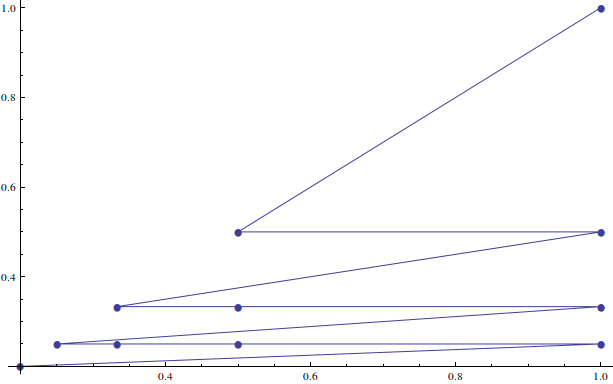
\includegraphics[scale=0.45]{countable_example1.png}
    \caption{\cref{c_exa1}}
\end{figure}
It is easy to see that $\{ \sigma^{n}((1,1)) \} = X \setminus X^{(1)}$.
\end{example}



\begin{lemma} \label{c_lam3}
   Let $X$ be a countably infinite, compact metric space such that $d(X)=2$
   and $X^{(2)} = \{c\}$. If $\{ \sigma^{n}(x) \}_{n=0}^{\infty}$ 
   is dense in $X$ for a isolated point $x$ in $X$, then $\sigma(c) = c$.
\end{lemma}

\begin{proof}
    Suppose that $\sigma(c) = y \in X^{(1)}$. If $y \neq c$, then $y$ is an
    isolated point in $X^{(1)}$. There exist a neighborhood $U$ of $c$ such
    that $\sigma(U) = \{ y \}$ and $X^{(1)} \setminus U$ contains only finite
    many points. By \cref{c_lam2}, there exist a $n$ such that $\sigma^{n}(y)
    \in U$, since no isolated point in $X^{(1)}$ is periodic. However
    we have $\sigma^{n+1}(y) = y$. It is a contradiction.
\end{proof}

Let $(X, \sigma)$ be a dynamic system, $A$ a subset of $X$ 
and $x$ a point in $X$. Let 
$A(x) = \{m : \sigma^{m}(x) \in A \mbox{, }\}$. Recall that 
the upper asymptotic density $\overline{d}(A(x))$ is 
$\limsup\limits_{n\rightarrow \infty} \frac{|A(x,n)|}{n}$ and 
lower asymptotic density $\underline{d}(A(x))$ is 
$\liminf \limits_{n\rightarrow \infty} \frac{|A(x,n)|}{n}$,
where $A(x,n) = \{1, 2, \ldots, n\} \cap A(x)$. $A(x)$ has 
asymptotic density $den(A(x))$ if $\overline{d}(A(x))=\underline{d}(A(x))$,
in which case $den(A(x))$ is equal to this common value.


\begin{lemma} \label{c_lam4}
   Let $X$ be a countably infinite, compact metric space such that $d(X) \geq 2$.
   Suppose that $\{ \sigma^{n}(x) \}_{n=0}^{\infty}$ 
   is dense in $X$ for a isolated point $x$ in $X$. Let $A = \{\sigma^{n_k}(x)\}$
   be a subsequence converge to $y$. If $y$ is not a periodic point, then 
   $den(A(x)) = 0$.
\end{lemma}

\begin{proof}
   We consider the following two cases.
   \begin{enumerate}
       \item $\sigma^{m_1}(y) \neq \sigma^{m_2}(y)$ if $m_1 \neq m_2$.
           Hence $\lim_{m \rightarrow \infty}\sigma^{m}(y) = c$. Fix a positive
           integer $k$. We choose $k+1$ neighborhoods $\{U_i \}_{i=0}^{k}$ of 
           $\sigma^{i}(y)$ such that $U_{i} \cap U_{j} = \varnothing$ and 
           $\sigma(U_i) \subset U_{i+1}$. Note that $A \setminus U_{0}$ contains 
           finite many points. Therefore there exists a $l \in \N$ such that 
           $\{\sigma^{n}(x) : n \geq l\}$ do not contains any element in 
           $A \setminus U_{0}$. If $n \geq l$ and $n \in A(x)$, we have
           $n+1, \ldots n+k$ are not in $A$. It is easy to see that
           $\overline{d}(A(x)) \leq \frac{1}{k}$. Hence $den(A(x)) = 0$. 
       \item $\sigma^{m}(y) = c_0$ and $c_0$ is a periodic point such that 
           $\sigma^{j}(c_0) = c_{j}$ and $\sigma^{n}(c_0) = c_0$. 
           Fix a positive integer $k$. We choose
           $m$ neighborhoods $U_i$ of $\sigma^{i}(y)$ for $i = 0, \ldots, m-1$
           and $k$ neighborhoods $\{U_{m + nl+ j} \}_{l=0}^{k-1}$ of $c_j$, 
           $j = 0, \ldots, n-1$ such that
           \begin{itemize}
               \item $U_{m + nl+ j}\subset U_{m + n(l+1)+ j}$, $l = 0, \ldots, k-1$,
                \item $U_{i_1} \cap U_{i_2} = \varnothing$ 
                    for $i_1 \neq i_2$ and $i_1, i_2 \in
                    \{0, \ldots, m-1\}$, 
                \item $U_i \cap U_{m + nk+ j} = \varnothing$ for 
                    $i = 0, \ldots, m-1$ and $j = 0 \ldots n-1$,
                \item $U_{m + nk+ j_1} \cap U_{m + nk+ j_2}= \varnothing$ 
                    for $j_1 \neq j_2$,
                \item $\sigma(U_i) \subset U_{i+1}$ for $i = 0, 1, \ldots, m+nk-1$.
            \end{itemize} 
           Note that $A \setminus U_{0}$ contains 
           finite many points. Therefore there exists a $N_0 \in \N$ such that 
           $\{\sigma^{n}(x) : n \geq N_0\}$ do not contains any element in 
           $A \setminus U_{0}$. If $s \geq N_0$ and $s \in A(x)$, we have
           $s+1, \ldots s+nk+m-1$ are not in $A$. It is easy to see that
           $\overline{d}(A(x)) \leq \frac{1}{nk+m-1}$. Hence $den(A(x)) = 0$ 
    \end{enumerate}
\end{proof}

\begin{corollary} \label{c_cor1}
   Let $X$ be a countably infinite, compact metric space such that $d(X)=2$
   and $X^{(2)} = \{c\}$. Suppose that $\{ \sigma^{n}(x) \}_{n=0}^{\infty}$ 
   is dense in $X$ for a isolated point $x$ in $X$. Let $B$ be any neighborhood
   of $c$ and $A = X \setminus B$. Then $den(A(x)) = 0$.
\end{corollary}

\begin{proof}
    Note that $A \cap X^{(1)}$ contains finite elements $\{c_1, \ldots, c_m \}$.
    Since $A$ is closed, $A=\cup^{m}_{k=1}A_{k}$, where $A_{k}$ is a 
    subsequence of $\{\sigma^{n}(x)\}$ converges to $c_k$. Each $c_k$ is not
    periodic by \cref{c_lam2}. Then
    $den(A_{k}(x)) = 0$ by \cref{c_lam4},. Therefore $den(A(x)) = 0$.
\end{proof}

\begin{corollary} \label{c_cor2}
    Let $(X, \sigma)$ be a dynamic system and $x \in X$. Let $Y$ be the closure of  
    $\{ \sigma^{n}(x) \}_{n=0}^{\infty}$. If $d(Y) = 2$ and $Y^{(2)} = \{c\}$, 
    then $\lim_{N \rightarrow \infty}
   \frac{1}{N} \sum_{n \leq N}\mu(n)f(\sigma^{n}(x)) = 0$ for any $f \in C(X)$.
\end{corollary}

\begin{proof}
    We could assume that $f(c) = 0$. For any $\varepsilon > 0$, there is 
    neighborhood $U$ of $c$ such that $|f(y)|< \varepsilon$ for any $y \in U$.
    By \cref{c_cor1}, $den(A(x)) = 0$ where $A = \{\sigma^{n}(x) : 
    \sigma^{n}(x) \mbox{ not in } U \}$. This implies the result. 
\end{proof}

\begin{example} \label{c_exa2}
    Let
    \begin{align*}
        X_1 &= \bigcup^{\infty}_{n=1} (\{ (2+\frac{1}{n}, \frac{1}{n+k}):
        k = 0,1, 2, \ldots \} \bigcup \{(2+\frac{1}{n},0)\})
        \bigcup \{(2,0)\},\\
        X_2 &= \bigcup^{\infty}_{n=2} (\{ (\frac{1}{n}, \frac{1}{n+k}):
        k = 0,1, 2, \ldots \} \bigcup \{(\frac{1}{n},0)\}) 
        \bigcup \{ (1, \frac{1}{2+k}):
        k = 0,1, 2, \ldots \} \bigcup \{(\frac{1}{n},0)\}
        \bigcup \{(0,0)\},\\
    \end{align*}
    $X = X_1 \cup X_2$.
    Then $X^{(1)} = \{(\frac{1}{n},0): n = 1, 2, \ldots \}
    \cup \{(0,0)\} \cup \{(2+\frac{1}{n},0): n = 1, 2, \ldots \}
    \cup \{(2,0)\}$ and $X^{(2)} = \{(0,0)\} \cup \{(2,0)\}$.
    Let $\sigma$ be a map $X \rightarrow X$ defined by
    \begin{align*}
        & (3,0) \rightarrow (0,0) \mbox{ and } (2,0) \rightarrow (2,0) \\
        & (1,0) \rightarrow (2,0) \mbox{ and } (0,0) \rightarrow (0,0) \\
        & (2+\frac{1}{n}, 0) \rightarrow (2+\frac{1}{n-1}, 0) \qquad 
        \mbox{(for $n > 1$)}\\
        & (\frac{1}{n}, 0) \rightarrow (\frac{1}{n-1}, 0) \qquad 
        \mbox{(for $n > 1$)}\\
        &(3, \frac{1}{k+1}) \rightarrow (\frac{1}{k+2}, \frac{1}{k+2})\\
        &(1, \frac{1}{2+k}) \rightarrow (2+\frac{1}{k+2}, \frac{1}{k+2})\\
        &(2+\frac{1}{n}, \frac{1}{n+k}) \rightarrow  
        (2+\frac{1}{n-1}, \frac{1}{n+k}) \qquad \mbox{(for $n > 1$).} \\
        &(\frac{1}{n}, \frac{1}{n+k}) \rightarrow  
        (\frac{1}{n-1}, \frac{1}{n+k}) \qquad \mbox{(for $n > 1$).} \\
    \end{align*}
    It is easy to see that $\{ \sigma^{n}((3,1)) \} = X \setminus X^{(1)}$.
    Let
    \begin{align*}
        \mathcal{X}(n) =  
        \begin{cases}
            1  \mbox{, $n \in [m^2 -m +1, m^{2}]$ for $m = 1, 2, \ldots$}\\
            0  \mbox{, $n \in [m^2 + 1 , m(m+1)]$ for $m = 1, 2, \ldots$}\\
         \end{cases} 
    \end{align*}
\end{example}

\begin{figure}[h]
    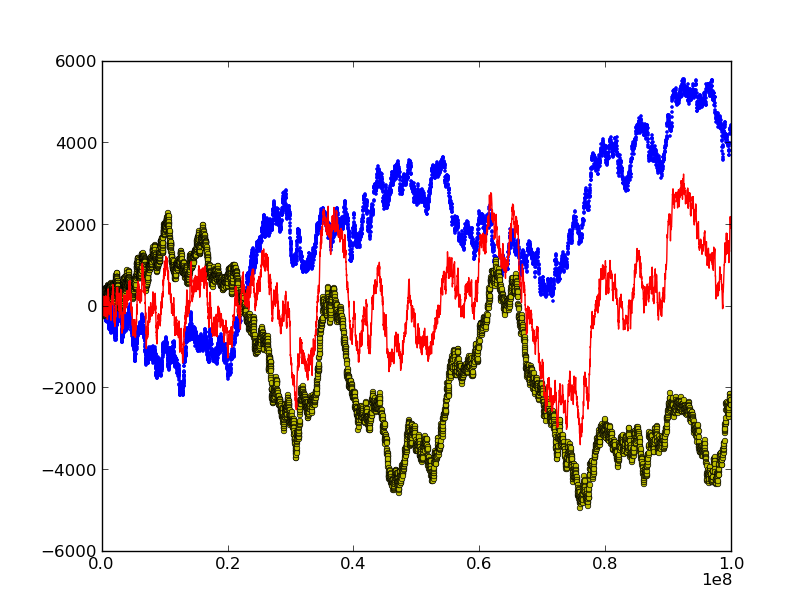
\includegraphics[scale=0.5]{100000000_all.png}
    \caption{\cref{c_exa2}, up to 100000000}
    \caption*{Blue: $\sum^{t}_{n} \mu(n)\mathcal{X}(n)$, max:$5561$, min:$
        -2197$.
        Yellow: $\sum^{t}_{n} \mu(n)(1-\mathcal{X}(n))$, max:$2278$, min:$
        -4954$. 
        Red: $\sum^{t}_{n} \mu(n)$, max:$3225$, min:$-3402$.}
\end{figure}

\begin{figure}[h]
    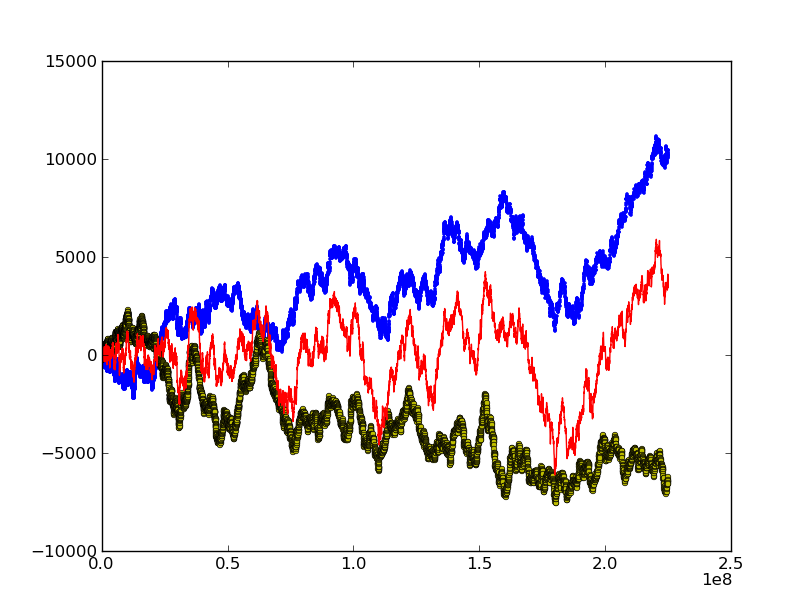
\includegraphics[scale=0.5]{225000000_all.png}
    \caption{\cref{c_exa2}, up to 225000000}
    \caption*{Blue: $\sum^{t}_{n} \mu(n)\mathcal{X}(n)$, max:$11175$, min:$
        -2197$.
        Yellow: $\sum^{t}_{n} \mu(n)(1-\mathcal{X}(n))$, max:$2278$, min:$
        -7547$. 
        Red: $\sum^{t}_{n} \mu(n)$, max:$5890$, min:$-6136$.}
\end{figure}

\begin{figure}[h]
    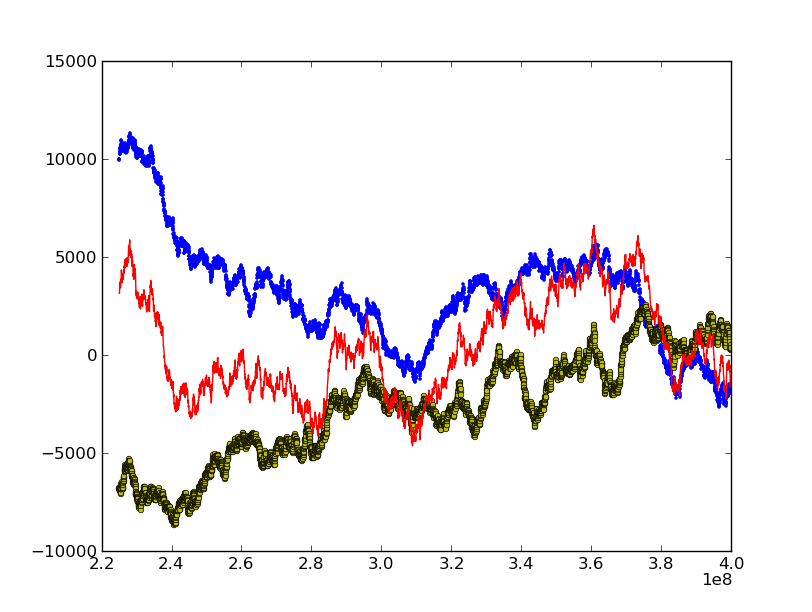
\includegraphics[scale=0.5]{400000000_all.png}
    \caption{\cref{c_exa2}, up to 400000000}
    \caption*{Blue: $\sum^{t}_{n} \mu(n)\mathcal{X}(n)$, max:$11319$, min:$
        -2663$.
        Yellow: $\sum^{t}_{n} \mu(n)(1-\mathcal{X}(n))$, max:$2527$, min:$
        -8688$. 
        Red: $\sum^{t}_{n} \mu(n)$, max:$6602$, min:$-4645$.}
\end{figure}

In number theory, the Mertens function $M(x)$ is defined as 
\begin{align*}
    M(x) = \sum_{k \leq x}\mu(k). 
\end{align*}


By Theorem 333 in \cite{HW}, the probabilit that a number should be squarefree is
$\frac{6}{\pi^2}$, more precisely
\begin{align*}
    Q(x) = \sum_{n \leq x}|\mu(n)| = \frac{6x}{\pi^2} + O(\sqrt{x}).
\end{align*}

\begin{lemma}\label{c_lam6}
   \begin{align*}
       \sum_{n \leq x} \X(n)\log n = \frac{x}{2}logx + O(x).
   \end{align*} 
\end{lemma}

\begin{proof}
    Let $x = m^2 + m + l$ where $0 \leq l < 2(m+1)$. 
    Note
    \begin{align*}
        \sum_{n \leq x} (1-\X(n))\log n - \X(n)\log n &= 
        \sum^{m}_{k=1} \sum_{i=1}^{k}\log(\frac{k^2+ i}{k^{2}-k +i})
        +\sum_{j=m^2+m+1}^{m^2+m+l} \log(j) \\
        &=\sum^{m}_{k=1} \sum_{i=1}^{k} O(\frac{1}{k}) +  O(\sqrt{x}\log x)
        = O(\sqrt{x}\log x).
    \end{align*}
    By Theorem 423 in \cite{HW}, 
    \begin{align*}
        \sum_{n \leq x} \log n =\sum_{n \leq x} (1-\X(n))\log n + \X(n)\log n 
        = x\log x + O(x).
    \end{align*}
    Therefore
    \begin{align*}
        \sum_{n \leq x} \X(n)\log n = \frac{x}{2}logx + O(x).
    \end{align*} 
\end{proof}

\begin{lemma}\label{c_lam7}
    Let $S_{l} = \bigcup_{m=1}^{\infty}
    \{l\times m^2 + t : t \in [0, lm] \}$.
    If $j/i = k^2 > 1$, then
    \begin{align*}
        \lim_{x \rightarrow \infty} 
        \frac{\# \{n \leq x: n \in S_{i} \cap S_{j}\}}{x} = 
        \begin{cases}
            \frac{k+1}{4k} &\mbox{ if $k$ is odd}\\
            \frac{1}{4} &\mbox{ if $k$ is even}
        \end{cases}. 
    \end{align*}
\end{lemma}

\begin{proof}
   Assume that $x = ka$ and $y = a$. Then $ix^2 = ik^2 a^2 = ja^2 = jy^2$. 
   Consider the interval 
   \begin{align*}
        s_y = [jy^2, j(y+1)^2 -1] = [jy^2, jy^2 + jy] 
        \cup [jy^2 + jy + 1, j(y+1)^2 -1] = s_{y}^{1} + s_{y}^{2}.   
   \end{align*} 
   Note that $[jy^2, j(y+1)^2-1]$ contains $k$ intervals
   \begin{align*}
       [ix^2, ix^2+ix], [i(x+1)^2, i(x+1)^2 + i(x+1)], \ldots, 
       [i(x+k-1)^2, i(x+k -1)^2+ i(x+ k-1)].
   \end{align*}

   If $k$ is even, then 
        \begin{align*}
            [ix^2, ix^2+ix], [i(x+1)^2, i(x+1)^2 + i(x+1)], \ldots, 
            [i(x+\frac{k}{2}-1)^2, i(x+\frac{k}{2} -1)^2+ i(x+ \frac{k}{2}-1)]
        \end{align*}
        are in $s_{y}^{1}$ for $x$ large enough, 
        since $i(x + \frac{k}{2} - \frac{k^2}{4}) >0$. And
            \begin{align*}
            [i(x+\frac{k}{2})^2, i(x+\frac{k}{2})^2+ i(x+ \frac{k}{2})], \ldots,
            [i(x+k-1)^2, i(x+k-1)^2+ i(x+k-1)]
        \end{align*}
        are in $s_{y}^2$. This implies that 
        $\lim_{x \rightarrow \infty} 
        \frac{\# \{n \leq x: n \in S_{i} \cap S_{j}\}}{x} = \frac{1}{4}$. 

    If $k$ is odd, then
    \begin{align*}
        i(x+\frac{k-1}{2})^2+ i(x+ \frac{k-1}{2}) -jy^2 -jy = \frac{i(k^2-1)}{4}. 
    \end{align*}
    Therefore $s_{y}^{1}$ contains almost $\frac{k+1}{2}$ intervals. It is clear
    imples the result.
\end{proof}



\begin{lemma}\label{c_lam8}
    Suppose that $p$, $q$ are two coprime positive integers, 
    i.e. $(p,q) = 1$. Let 
    $S_1 = \bigcup^{p}_{k=1}[\frac{(2k-2)}{2p}, \frac{(2k-1)}{2p}]$ and
    $S_2 = \bigcup^{q}_{k=1}[\frac{(2k-2)}{2q},\frac{(2k-1)}{2q}]$. 
    \begin{align*}
        len(S_1 \cap S_2) = 
        \begin{cases}
            \frac{1}{4} & \mbox{if $p$ or $q$ is even},\\
            \frac{1}{4} + \frac{4}{15pq} & \mbox{otherwise.}
        \end{cases}
    \end{align*}
\end{lemma}

\begin{proof}
    Let $\X_{1}$ and $\X_{2}$ be the charachteristic function of $S_1$
    and $S_2$ respectively.
    \begin{align*}
        \langle \X_1, e^{2\pi in \theta}\rangle &= 
        \sum_{k=1}^{p}
        \int_{\frac{2k-2}{2p}}^{\frac{2k-1}{2p}} e^{-2\pi in \theta}\\
        &=\frac{1-e^{\frac{-\pi in}{p}}}{2\pi in}
        \sum_{k=0}^{p-1}e^{\frac{-2\pi ink}{p}} 
        = \begin{cases}
             \frac{1}{2} & n = 0\\
             \frac{p}{\pi i n}, & \mbox{if } n = p(2a + 1), a \in \Z \\
             0, & \mbox{otherwise}
          \end{cases}.
    \end{align*}
    Similiarly,
    \begin{align*}
        \langle \X_2, e^{2\pi in \theta}\rangle &= 
        \sum_{k=1}^{q}
        \int_{\frac{2k-2}{2q}}^{\frac{2k-1}{2q}} e^{-2\pi in \theta}\\
        &=\frac{1-e^{\frac{-\pi in}{q}}}{2\pi in}
        \sum_{k=0}^{q-1}e^{\frac{-2\pi ink}{q}} 
        = \begin{cases}
             \frac{1}{2} & n = 0\\
              \frac{q}{\pi i n}, & \mbox{if } n=q(2a + 1), a \in \Z  \\
              0, & \mbox{otherwise} 
          \end{cases}
    \end{align*}
    If $p$ or $q$ is even, then $\langle \X_1, \X_2 \rangle = \frac{1}{4}$.
    If both $p$ and $q$ are odd, then
    \begin{align*}
        len(S_1 \cap S_2)&=\langle \X_1, \X_2 \rangle \\
        &= \frac{1}{4} + \frac{1}{\pi^2 pq}
        \sum_{k \in \Z }^{\infty}\frac{1}{(2k+1)^2}\\ 
        &= \frac{1}{4} + \frac{8}{5\pi^2 pq}\zeta(2)
         = \frac{1}{4} + \frac{4}{15pq}
        \qquad (\zeta(2) = \frac{\pi^2}{6}).\\
    \end{align*} 
\end{proof}

\begin{theorem}[Dirichlet, c. 1840]
   For any real number $k$ and any integer $N \geq 1$, there exist
   integers $p$ and $q$ such that $1 \leq q \leq N$ and 
   \begin{align*}
       |qk - p| \leq \frac{1}{N+1}. 
   \end{align*}
\end{theorem}

\begin{lemma}\label{c_lam9}
    Let $S_{l} = \bigcup_{m=1}^{\infty}
    \{l\times m^2 + t : t \in [0, lm] \}$.
    If $\sqrt{\frac{i}{j}}  \in \R \setminus \Q$, then
    \begin{align*}
        \lim_{x \rightarrow \infty} 
        \frac{\# \{n \leq x: n \in S_{i} \cap S_{j}\}}{x} = \frac{1}{4}.
    \end{align*}
\end{lemma}

\begin{proof}
   We assume that $\sqrt{\frac{i}{j}} < 1$ and 
   $|\sqrt{\frac{i}{j}}q - p| \leq \frac{1}{q}$.
   Since
   \begin{align*}
       \lim_{m \rightarrow \infty} \frac{iq^2l^2}{iq^2(l+1)^2} = 1, 
   \end{align*}
   we only need to consider the case for $x = iq^2l^2$, where $l \in \N$. 
   The interval $[iq^2l^2, iq^2(l+1)^2]$  
   contains $q$ invervals in $S_1$: 
   \begin{align*}
       [i(ql)^2, i((ql)^2 + ql)], \ldots,  [i(ql+q-1)^2, i(ql+q)(ql+q-1)].
   \end{align*}
   Let 
   \begin{align*}
       S_{1l} &= \bigcup_{k=1}^{q} [i(ql+k-1)^2, i(ql+k)(ql+k-1)]\\ 
       S_{1l}' &= \bigcup_{k=1}^{q} [i(ql)^2+(2k-2)iql, i(ql)^2+(2k-1)iql].
   \end{align*} 
   Note that
   \begin{align*}
       \lim_{l \rightarrow 0}\frac{\# (S_{1l} \cap S_{1l}')}{iq^2l} = 1. 
   \end{align*}
   If $iq^2l^2 \leq jy^2 \leq iq^2(l+1)^2$, then 
   \begin{align*}
       \sqrt{\frac{i}{j}}ql \leq y \leq \sqrt{\frac{i}{j}}q(l+1). 
   \end{align*}
   Since
   \begin{align*}
       p - \frac{1}{q} \leq \sqrt{\frac{i}{j}}q \leq p + \frac{1}{q}, 
   \end{align*}
   $[iq^2l^2, iq^2(l+1)^2]$ contains at least $p-3$ and at most $p+1$ intervals in
   $S_2$. Let $y_0$ be the first $y$ such that 
   $iq^2l^2 \leq jy^2 \leq iq^2(l+1)^2$. Let 
   \begin{align*}
       S_{2l} = \bigcup_{k=1}^{p-3}[j(y_0 + k-1)^2, j(y_0+k-1)^2+j(y_0+k-1)] 
       \subset S_2 \cap [iq^2l^2, iq^2(l+1)^2].
   \end{align*}
   Note that 
   \begin{align*}
       \liminf\limits_{l \rightarrow \infty}\frac{\# S_{2l}}
       {\#(S_2 \cap [iq^2l^2, iq^2(l+1)^2])} \geq 1 - \frac{5}{p-3}.
   \end{align*}
   Let 
   \begin{align*}
       S_{2l}' = \bigcup_{k=1}^{p-3}[jy_{0}^2 + (2k-2)jy_{0}, 
       jy_{0}^{2}+(2k-1)jy_{0}].
   \end{align*}
   Also we have
   \begin{align*}
       \lim_{l \rightarrow \infty} \frac{\# (S_{2l} \cap S_{2l}')}{iq^2l} = 1. 
   \end{align*}
   We would like to compare $S_{1l}'$ with $S_{2l}'$.
   Since $y_0 \leq \sqrt{\frac{i}{j}}ql +1$, we have
   \begin{align*}
       \Delta &= i(ql)^2 + 2iq^2l - jy_{0}^2 + (2p-7)jy_0\\ 
       &\geq i(ql)^2 + 2iq^2l - j(\sqrt{\frac{i}{j}}ql +1)^2
       + (2p -7)j(\sqrt{\frac{i}{j}}ql +1)\\
       & = 2iq^2l(1 - (\frac{p}{q}-\frac{5}{2q})\sqrt{\frac{j}{i}} 
       - \frac{(2p - 6)j}{2iq^2l})\\ 
       & \geq 2iq^2l(1 - (\sqrt{\frac{i}{j}} + \frac{1}{q^2} - \frac{5}{2q}) 
       \sqrt{\frac{j}{i}} - \frac{(2p - 6)j}{2iq^2l}) \qquad 
       (\frac{p}{q} \leq \sqrt{\frac{i}{j}} + \frac{1}{q^2})\\
        & = 2iq^2l((\frac{5}{2q}- \frac{1}{q^2}) 
        \sqrt{\frac{j}{i}} - \frac{(2p - 6)j}{2iq^2l}) \geq 0,
   \end{align*}
   provide that $l$ is large enough.
   
   This means that $S_{2l}'$ is contains in $[i(ql)^2, i(ql)^2 + 2iq^2l]$.
   A similar caculation as in the proof of \cref{c_lam9} shows that 
   \begin{align*}
       \lim_{l \rightarrow \infty} \frac{\#(S_{1l}' \cap S_{2l}')}{2iq^2l} = 
       \frac{1}{4} + O(\frac{1}{pq}).
   \end{align*}
   Therefore 
   \begin{align*}
       \lim_{l \rightarrow \infty} \frac{\#(S_{1l} \cap S_{2l})}{2iq^2l}
       = \frac{1}{4} + O(\frac{1}{p}).
   \end{align*}
   This implies that
    \begin{align*}
        \lim_{x \rightarrow \infty} 
        \frac{\# \{n \leq x: n \in S_{i} \cap S_{j}\}}{x} = \frac{1}{4} 
        + O(\frac{1}{p}).
    \end{align*}
   By increasing $p$ and $q$, the result is proved.
\end{proof}

\begin{lemma}
    Let $S_{l} = \bigcup_{m=1}^{\infty}
    \{l\times m^2 + l\times i : i \in [0, m] \}$.
    If $\sqrt{\frac{i}{j}}  \in \R \setminus \Q$, then
    \begin{align*}
        \lim_{x \rightarrow \infty} 
        \frac{\# \{n \leq x: n \in S_{i} \cap S_{j}\}}{x} = \frac{1}{4ij}
        \qquad (i \neq j). 
    \end{align*}
\end{lemma}

\begin{proof}
   
\end{proof}

\begin{theorem}[Carleson's theorem]
    Let $f$ be an $L^{p}$ periodic function for some $p \in (1, \infty)$,
    with Foruier coefficient $\hat{f}(n)$. Then
    \begin{align*}
        \lim_{N \rightarrow \infty}\sum_{|n|\leq N}
        \hat{f}(n)e^{2\pi inx} = f(x) 
    \end{align*}
    for almost every $x$.
\end{theorem}

\begin{figure}[h]
    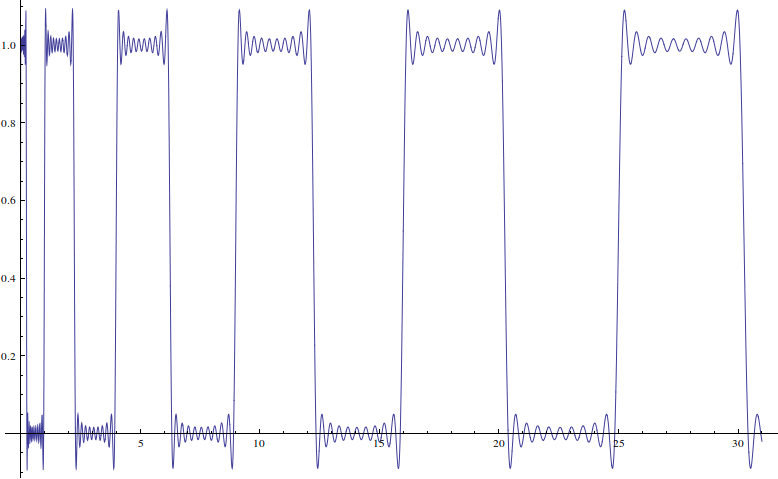
\includegraphics[scale=0.3]{fourier_converges.png}
    \caption{$\frac{1}{2} + \sum_{k=1}^{10}
    \frac{2}{(2k-1)\pi}\sin(2\pi i (2k-1)\sqrt{x})$, ($x \in [0, 31]$)}
\end{figure}

\begin{definition}
    A function $f(x)$ is piecewise continuous on an interval $I$ if
    it is continuous on $I$ except perhaps for a finite number of points,
    and if $a \in I$ is a point of discontinuity for $f(x)$ then 
    $f(a_{+})$ and $f(a_{-})$ exist: that is 
    \begin{align*}
        f(a_{+}) = \lim_{x \rightarrow a_{+}}f(x), \qquad 
        f(a_{-}) = \lim_{x \rightarrow a_{-}}f(x)
    \end{align*}
    are required to exist. We denote the space of piecewise continuous
    functions on $I$ by $E(I)$.
\end{definition}

\begin{definition}
    The space $E'$ is defined as the space of all functions $f(x) \in 
    E([-\pi, \pi]$
    such that the right-hand derivative $D_{+}f(x)$ and left-hand
    derivative $D_{-}f(x)$ exists. Recall that
    \begin{align*}
        D_{+}f(x) &= \lim_{h \rightarrow 0_{+}}\frac{f(x+h)-f(x_{+})}{h}\\ 
        D_{-}f(x) &= \lim_{h \rightarrow 0_{-}}\frac{f(x+h)-f(x_{-})}{h}.
    \end{align*}
\end{definition}

\begin{theorem}
   If $f \in E'$, then the Fourier series of $f$
   \begin{align*}
      \frac{a_{0}}{2} + \sum_{k = 1}^{\infty}(a_{k}\cos kx + b_{k}\sin kx), 
   \end{align*}
   where
   \begin{align*}
       a_{k} = \frac{1}{\pi}\int^{\pi}_{-\pi}f(x)\cos kx dx, \qquad
       b_{k} = \frac{1}{\pi}\int^{\pi}_{-\pi}f(x)\sin kx dx,
   \end{align*}
   converges pointwise to 
   \begin{align*}
       \frac{f(x_{+}) + f(x_{-})}{2}. 
   \end{align*}
\end{theorem}

\begin{theorem}
   Suppose that 
   \begin{itemize}
       \item $f(x)$ is continuous on $[-\pi, \pi]$
       \item $f(-\pi) = f(\pi)$
       \item $f'(x) \in E([-\pi, \pi])$.
   \end{itemize}
   Then
   \begin{align*}
      \frac{a_{0}}{2} + \sum_{k = 1}^{\infty}(a_{k}\cos kx + b_{k}\sin kx)
   \end{align*}
   converges uniformly to $f(x)$ on $[-\pi, \pi]$. 
\end{theorem}

\begin{corollary}
    Let $\X$ be the characteristic function of 
    $\bigcup_{m=1}^{\infty}[m^2, m^2+m+\frac{1}{4}]$.
    Then
    \begin{align*}
        \X = \frac{1}{2} + \sum_{k=1}^{\infty}
        \frac{2}{(2k-1)\pi}\sin(2\pi(2k-1)\sqrt{x}) 
        \qquad (\mbox{$x \geq 1$}) 
    \end{align*}
    at every point where $\X$ is continuous.
\end{corollary}


\begin{lemma} \label{Le_BSZ} [Bourgain-Sarnak-Ziegler]
Let $F: \mathbb{N} \rightarrow \mathbb{C}$ with $|F|\leq 1$ and 
let $\nu$ be a multiplicative function with $|\nu|\leq 1$. Let $\tau>0$ 
be a small parameter and assume that for all primes 
$p_1,p_2\leq e^{1/\tau}$, $p_1\neq p_2$, we have that for $M$ 
large enough
\[
\left|\sum_{m\leq M} F(p_1m)\overline{F(p_2m)}\right|\leq \tau M.
\]
Then for $N$ large enough
\[
\left|\sum_{n\leq N} \nu(n) F(n)\right| \leq 2 N \sqrt{\tau \log (1/\tau)}.
\]
\end{lemma}


\begin{lemma} [Kusmin-Landau] \label{Le_Kus-Lan}
If $f$ is continuously differentiable, $f^\prime$ is monotonic, and $0<\lambda\leq f^\prime(x)\leq 1-\lambda$ on the interval $(a,b]$, then
\[
\left|\sum_{a<n\leq b}e(f(n))\right|\ll \lambda^{-1}.
\]
\end{lemma}

\begin{lemma} \label{Le_multi_exponential}
Let $0<\gamma<1$. For arbitrarily small $\tau>0$, and for 
$0\neq |k|\leq x^{(1-\gamma)/2}$ and multiplicative function 
$\nu$ with $|\nu|\leq 1$, we have
\[
\left|\sum_{n\leq x} \nu(n) e(kn^\gamma)\right| \ll_\tau x
\]
\end{lemma}

\begin{proof}
With the help of Lemma \cref{Le_BSZ}, if we prove that for all 
primes $p_1\neq p_2\ll e^{1/\tau}$, the estimate
\[
\left|\sum_{n\leq x} e(k(p_1n)^\gamma -k (p_2 n)^\gamma)\right| \ll_\tau x
\]
holds for sufficiently large $x$, then
\[
\left|\sum_{n\leq x} \nu(n) e(kn^\gamma)\right| \ll_\tau x
\]
also holds. Since
\[
\left|\sum_{n\leq x(\log x)^{-1}} e(k(p_1n)^\gamma -k (p_2 n)^\gamma)
\right| \ll x(\log x)^{-1} \ll_\tau x
\]
for $x$ sufficiently large, it is sufficient to prove
\[
\left|\sum_{x(\log x)^{-1}\leq n\leq x} e(k(p_1n)^\gamma 
-k (p_2 n)^\gamma)\right| \ll_\tau x
\]
Take $f(n):=k(p_1^\gamma -p_2 ^\gamma) n^\gamma$ in Lemma \cref{Le_Kus-Lan}.
Note that
\[
|f^\prime(n)|\asymp k (p_1^\gamma -p_2 ^\gamma) n^{\gamma-1} 
\gg_\tau |k| x^{\gamma-1}
\]
and
\[
|f^\prime(n)|\asymp k (p_1^\gamma -p_2 ^\gamma) n^{\gamma-1} 
\ll_\tau |k| x^{\gamma-1} (\log x)^{1-\gamma}=\textit{o}_\tau(1)
\]
when $k\leq x^{(1-\gamma)/2}$. By Lemma \cref{Le_Kus-Lan}, we conclude that
\[
\left|\sum_{x(\log x)^{-1}\leq n\leq x} e(k(p_1n)^\gamma 
-k (p_2 n)^\gamma)\right| \ll_\tau x^{1-\gamma}.
\]
\end{proof}

\begin{theorem}
Let $0<\gamma<1$ and write $\beta=\gamma^{-1}$. 
Define $A=\bigcup_{m=1}^\infty [m^\beta, (m+\gamma)^\beta)$. 
Then for any multiplicative function $\nu$ with $|\nu|\leq 1$, we have
\[
\sum_{ n\leq x} \nu(n) 1_A(n) = \gamma \sum\limits_{n\leq x} \nu(n) 
+ \textit{o}(x).
\]
In particular, we have
\[
\sum_{ n\leq x} \mu(n) 1_A(n) = \textit{o}(x)
\]
and
\[
\sum_{ n\leq x} \mu^2(n) 1_A(n) = \frac{6\gamma}{\pi^2} x + \textit{o}(x).
\]
\end{theorem}

\begin{proof}
Let $\tau>0$ be an arbitrarily small parameter to be determined later. 
Define
\[
\widetilde{A}=\bigcup_{m=1}^\infty [m,m+\gamma]
\]
and
\[
\eta(y)=
\begin{cases}
\exp\left(-\frac{1}{1-\left((y-\tau-m)/\tau\right)^2}+1\right), 
\quad &y\in \bigcup_{m=1}^\infty [m,m+\tau),\\
1, \quad &y\in \bigcup_{m=1}^\infty [m+\tau,m+\gamma-\tau),\\
\exp\left(-\frac{1}{1-\left((y-\gamma+\tau-m)/\tau\right)^2}+1\right), 
\quad &y\in \bigcup_{m=1}^\infty [m+\gamma-\tau, m+\gamma),\\
0, \quad &y\in \bigcup_{m=1}^\infty [m+\gamma, m+1).
\end{cases}
\]
The function $\eta$ has the Fourier expansion
\[
\eta(y) = \sum_{k\in \Z} \widehat{\eta}(k) e(ky), \quad y\geq 1,
\]
where the Fourier coefficients 
$\widehat{\eta}(k)=\int_0^1 \eta(t)e(-kt) dt$ 
satisfy $|\widehat{\eta}(k)|\ll_{\tau,A} (2+|k|)^{-A}$. 
Write $\delta=(1-\gamma)/2$, we have
\begin{align*}
\eta(y) &= \sum_{|k|\leq x^{\delta/2}} \widehat{\eta}(k) e(ky)+ 
    \textit{O}_{\tau,A}\left(\sum_{|k|\geq x^{\delta/2}}|k|^{-A}\right)\\
&= \sum_{|k|\leq x^{\delta/2}} \widehat{\eta}(k) e(ky)
    + \textit{O}_{\tau,A}\left(x^{-100}\right).
\end{align*}

Now
\begin{align*}
&\sum_{ n\leq x} \nu(n) 1_A(n) = \sum_{  n\leq x} \nu(n) 
    1_{\widetilde{A}}(n^\gamma)\\
&\quad \quad \quad  = \sum_{  n\leq x} \nu(n) \eta(n^\gamma) 
    +\sum_{  n\leq x} \nu(n) \left(1_{\widetilde{A}}(n^\gamma)
    -\eta(n^\gamma)\right)\\
&\quad \quad \quad  := W_1+W_2.
\end{align*}

The first summation is
\begin{align*}
W_1&=\sum_{n \leq x} \nu(n) \left(\sum_{|k|\leq x^{\delta/2}} 
\widehat{\eta}(k) e(kn^\gamma) + \textit{O}_A\left(x^{-100}\right) 
\right)\\
&= \sum_{|k|\leq x^{\delta/2}} \widehat{\eta}(k) 
\left(\sum_{n \leq x} \nu(n) e(kn^\gamma)\right) 
+\textit{O}\left(1\right)\\
& = \widehat{\eta}(0) \sum_{n \leq x} \nu(n) 
+\textit{O}\left(1+\sum_{|k|\leq x^{\delta/2}}|\widehat{\eta}(k)| 
\left|\sum_{n \leq x} \nu(n) e(kn^\gamma)\right|\right)
\end{align*}

In view of Lemma \cref{Le_multi_exponential}, 
the summation in the error term is $\textit{O}_\tau(x)$. The coefficient
\[
\widehat{\eta}(0)=\int_0^1 \eta(y) dy = \gamma + \textit{O}(\tau).
\]
As a result, it follows that
\[
W_1 = \gamma \sum_{n\leq x}\nu(n)+ \textit{O}\left(\tau x\right).
\]

Now we start to bound $W_2$. 
Write $h(n)=1_{\tilde{A}}(n^\gamma)-\eta(n^\gamma)$, then
\[
\text{Supp}(h)\cap [1,x] \subseteq \bigcup_{m=1}^{x^\gamma} 
[m^\beta, (m+\tau)^\beta] \cup [(m+\gamma-\tau)^\beta, (m+\gamma)^\beta].
\]
Hence
\[
W_2 \ll \sum_{m\leq x^\gamma} \tau m^{\beta-1} \ll \tau x.
\]

Putting every thing together, we see that
\[
\sum_{ n\leq x} \nu(n) 1_A(n) =\gamma \sum_{n\leq x}\nu(n)
+ \textit{O}\left( \tau x\right).
\]
Since $\tau>0$ can be chosen arbitrarily small, it can be conclude that
\[
\sum_{ n\leq x} \nu(n) 1_A(n) =\gamma \sum_{n\leq x}\nu(n)+\textit{o}(x).
\]
\end{proof}

\begin{lemma}
   \begin{align*}
       \sum_{n \leq x}\left[\frac{x}{n} \right]\X(n)\Lambda(n) 
       = \frac{x}{2}\log x + O(x). 
   \end{align*} 
\end{lemma}

\begin{proof}
    Assume that $x = m^2+m$. We claim that 
    \begin{align*}
        \sum_{k=1}^{m} \sum_{l=1}^{k}\left[\frac{m^2+m}{k^2+l} 
        \right]\Lambda(k^2+l) 
        - \sum_{k=1}^{m} \sum_{l=1}^{k}\left[\frac{m^2+m}{k^2-k+l} \right]
        \Lambda(k^2-k+l) = O(x).
    \end{align*} 
    First note that
    \begin{align*}
        &\sum_{k=1}^{m} \sum_{l=1}^{k}\left[\frac{m^2+m}{k^2+l} 
        \right]\Lambda(k^2+l) 
        - \sum_{k=1}^{m} \sum_{l=1}^{k}\left[\frac{m^2+m}{k^2-k+l} \right]
        \Lambda(k^2-k+l) \\
        &=
        \sum_{k=1}^{m} \sum_{l=1}^{k}\frac{m^2+m}{k^2+l} 
        \Lambda(k^2+l) 
        - \sum_{k=1}^{m} \sum_{l=1}^{k}\frac{m^2+m}{k^2-k+l}
        \Lambda(k^2-k+l) + O(x).
    \end{align*}
    However
    \begin{align*}
        &\sum_{k=1}^{m} \sum_{l=1}^{k}(\frac{m^2+m}{k^2+l} - \frac{m^2+m}{k^2}) 
        \Lambda(k^2+l)\\
        &=x\sum_{k=1}^{m} \sum_{l=1}^{k}(\frac{-l}{k^2(k^2+l)})
        \Lambda(k^2+l)
        = xO(\sum_{k=1}^{m}\frac{\log 2k}{k^3}) = O(x). 
    \end{align*}
    Similarly
    \begin{align*}
        &\sum_{k=1}^{m} \sum_{l=1}^{k}(\frac{m^2+m}{k^2 -k +l} - \frac{m^2+m}{k^2}) 
        \Lambda(k^2-k+l)\\
        &=x\sum_{k=1}^{m} \sum_{l=1}^{k}(\frac{k-l}{k^2(k^2-k+l)})
        \Lambda(k^2-k+l)
        = xO(\sum_{k=1}^{m}\frac{\log 2k}{k^3}) = O(x). 
    \end{align*}
    Therefore, we only need to show
    \begin{align*}
        \sum_{k=1}^{m} \frac{m^2+m}{k^2}\sum_{l=1}^{k}\left (
        \left[\frac{k^2+k}{k^2+l}\right]\Lambda(k^2+l) -
    \left[\frac{k^2}{k^2-k+l}\right]\Lambda(k^2-k+l) \right)
    \end{align*}
\end{proof}

Let $\Psi_{\X}(k,x) = \sum_{d \leq x}\X(dk)\Lambda(d) \mbox{ and }
\Psi_{1-\X}(k,x) = \sum_{d \leq x}(1-\X(dk))\Lambda(d)$.

Recall that
\begin{align*}
    \Psi(x) = \sum_{d \leq x}\Lambda(d) = O(x).
\end{align*}
Therefore $\Psi_{\X}(k,x) = O(x)$ and $\Psi_{1-\X}(k,x) = O(x)$.

\begin{lemma}
    Let 
    \begin{align*}
        \Psi(k,x) = \sum_{d \leq x}\X(dk)\Lambda(d).
    \end{align*} 
    Then $\Psi(k,x) - \frac{1}{2}[x] = o(x)$.
\end{lemma}

\begin{proof}
   Let $\Psi(x) = \sum_{d \leq x}\Lambda(d) = \Psi(k,x)$ 
\end{proof}

\begin{lemma}
    Let $M_{\X}(x) = \sum_{n \leq x}\X(n)\mu(n)$. Then
    $M_{\X}(x) = o(x)$. 
\end{lemma}

\begin{proof}
    By Theorem 434 in \cite{HW}, we have
    \begin{align*}
        \sum_{n \leq x} \X(n)\mu(n)log(\frac{x}{n}) = O(x). 
    \end{align*}
    Hence
    \begin{align*}
        M_{\X}(x)log(x) = \sum_{n \leq x}\X(n)\mu(n)\log n + O(x).    
    \end{align*}
    By Theorem 297 in \cite{HW},
    \begin{align*}
        -\sum_{n \leq x}\X(n)\mu(n)\log n 
        &= \sum_{n \leq x}\X(n)\sum_{d | n}
        \mu(\frac{n}{d})\Lambda(d)
        = \sum_{dk \leq x}\X(dk)\mu(k)\Lambda(d)\\
        & = \sum_{k \leq x} \mu(k)\sum_{d \leq \frac{x}{k}}\X(dk)\Lambda(d)
    \end{align*}
\end{proof}

\begin{lemma}[Conjecture]
    Let $(X, \sigma)$ be a dynamic system where $X$ is a compact 
    Hausdorff metric space and $\iota(X)$ is the set of 
    all isolated points of $X$. Let $X' = X \setminus \iota(X)$. If
    $\sigma(X') \subset X'$ and $\lim_{N \rightarrow \infty}
       \frac{1}{N} \sum_{n \leq N}\mu(n)f(\sigma^{n}(x)) = 0$ for any
    $f \in C(X')$ and any $x \in X'$, then $\lim_{N \rightarrow \infty}
       \frac{1}{N} \sum_{n \leq N}\mu(n)f(\sigma^{n}(x)) = 0$ for any 
    $f$ in $C(X)$ and $x \in X$.
\end{lemma}

\section{Weighted Sum of $\mu(n)$}

Let $f: \N \rightarrow \N$ be a function defined on $\N$.
Consider the weighted sum
\begin{align*}
    \sum_{n \leq N}f(n)\mu(n) 
\end{align*}

Let $\rho: \N \rightarrow \N$ be a map defined by
\begin{align*}
\rho : p_{1}^{\gamma(1)}p_{2}^{\gamma(2)}\cdots p_{n}^{\gamma(n)} 
\rightarrow
1^{\gamma(1)}2^{\gamma(2)}\cdots n^{\gamma(n)}, 
\end{align*}
where $p_i$ is the $i$-th prime number.

\begin{remark}
    If $k< \sqrt{N}$, then $\floor{\frac{N}{k}} > \floor{\frac{N}{k+1}}$. 
    Assume that $N = ak + b$ where $0 \leq b < k$ and $a \geq k$. 
    If $\floor{\frac{N}{k}} = \floor{\frac{N}{k+1}}$, then
    $ak+ b = a(k+1)+c$. It is impossible.
\end{remark}

\begin{lemma}
 \begin{align*}
    \sum_{\gamma \in (\Z_{2})^{N} \mbox{ and } 
    1^{\gamma(1)}2^{\gamma(2)}\cdots N^{\gamma(N)} \leq M} 
    (-1)^{\sum_{i}\gamma(i)} = 0.
\end{align*}
\end{lemma}

\begin{proof}
  \begin{align*}
    &\sum_{\gamma \in (\Z_{2})^{N} \mbox{ and } 
    1^{\gamma(1)}2^{\gamma(2)}\cdots N^{\gamma(N)} \leq M} 
    (-1)^{\sum_{i}\gamma(i)} \\
    & = \sum_{\gamma \in (\Z_{2})^{N} \mbox{ and } 
    2^{\gamma(2)}\cdots N^{\gamma(N)} \leq M} 
    (-1)^{\sum_{i=2}^{N}\gamma(i)}
    - \sum_{\gamma \in (\Z_{2})^{N} \mbox{ and } 
    2^{\gamma(2)}\cdots N^{\gamma(N)} \leq M} 
    (-1)^{\sum_{i=2}^{N}\gamma(i)} \\
    &= 0.
\end{align*}
\end{proof}

Estimate
 \begin{align*}
    \sum_{\gamma \in (\Z_{2})^{N} \mbox{ and } 
    2^{\gamma(2)}\cdots N^{\gamma(N)} \leq N} 
    (-1)^{\sum_{i}\gamma(i)}.
\end{align*}

Note that if $j > \floor{\frac{N}{2}}$ and $\gamma(j) = 1$, 
    then $\gamma(i) = 0$ for any $i \neq j$. 
    Therefore
    \begin{align*}
        &\sum_{\gamma \in (\Z_{2})^{N} \mbox{ and } 
        2^{\gamma(2)}\cdots N^{\gamma(N)} \leq N} 
        (-1)^{\sum_{i}\gamma(i)}\\ 
        &= \sum_{\gamma \in (\Z_{2})^{\floor{\frac{N}{2}}} \mbox{ and } 
        2^{\gamma(2)}\cdots 
        (\floor{\frac{N}{2}})^{\gamma(\floor{\frac{N}{2}})} \leq N} 
        (-1)^{\sum_{i}\gamma(i)} - (N- \floor{\frac{N}{2}}). 
    \end{align*}


Similar argument implies that
\begin{align*}
    \sum_{\gamma \in (\Z_{2})^{\frac{N}{2}} \mbox{ and } 
    1^{\gamma(1)}2^{\gamma(2)}\cdots 
(\floor{\frac{N}{2}})^{\gamma(\floor{\frac{N}{2}})} \leq N} 
    (-1)^{\sum_{i}\gamma(i)}
=\sum_{\gamma \in (\Z_{2})^{\frac{N}{3}} \mbox{ and } 
    1^{\gamma(1)}2^{\gamma(2)}\cdots 
(\floor{\frac{N}{3}})^{\gamma(\floor{\frac{N}{3}})} \leq N} 
    (-1)^{\sum_{i}\gamma(i)}.
\end{align*}
Suppose that $\gamma(j) = 1$ and $\floor{\frac{N}{4}} < j \leq 
\floor{\frac{N}{3}}$.
The possibilities are
\begin{align*}
    &\gamma(1) = \gamma(2) = \gamma(3) = 0 \qquad 
    \gamma(1) = 1, \gamma(2) = \gamma(3) = 0 \\
    &\gamma(1) = 0, \gamma(2) = 1, \gamma(3) = 0 \qquad 
    \gamma(1) = 0, \gamma(2) = 0, \gamma(3) = 1 \\
    &\gamma(1) = 0, \gamma(2) = 0, \gamma(3) = 1 \qquad 
    \gamma(1) = 1, \gamma(2) = 1, \gamma(3) = 0 \\
    &\gamma(1) = 1, \gamma(2) = 0, \gamma(3) = 1.
\end{align*}
This implies that
\begin{align*}
    \sum_{\gamma \in (\Z_{2})^{\frac{N}{3}} \mbox{ and } 
    1^{\gamma(1)}2^{\gamma(2)}\cdots 
(\floor{\frac{N}{3}})^{\gamma(\floor{\frac{N}{3}})} \leq N} 
    (-1)^{\sum_{i}\gamma(i)}
=\sum_{\gamma \in (\Z_{2})^{\frac{N}{4}} \mbox{ and } 
    1^{\gamma(1)}2^{\gamma(2)}\cdots 
(\floor{\frac{N}{4}})^{\gamma(\floor{\frac{N}{4}})} \leq N} 
    (-1)^{\sum_{i}\gamma(i)}
\end{align*}
Similarly, we have
\begin{align*}
    \sum_{\gamma \in (\Z_{2})^{\frac{N}{4}} \mbox{ and } 
    1^{\gamma(1)}2^{\gamma(2)}\cdots 
(\floor{\frac{N}{4}})^{\gamma(\floor{\frac{N}{4}})} \leq N} 
    (-1)^{\sum_{i}\gamma(i)}
    =\sum_{\gamma \in (\Z_{2})^{\frac{N}{6}} \mbox{ and } 
    1^{\gamma(1)}2^{\gamma(2)}\cdots 
(\floor{\frac{N}{6}})^{\gamma(\floor{\frac{N}{6}})} \leq N} 
    (-1)^{\sum_{i}\gamma(i)}
\end{align*}

Assume that $k + 1 \leq \sqrt{N}$ and 
\begin{align*}
    \sum_{\gamma \in (\Z_{2})^{N} \mbox{ and } 
    1^{\gamma(1)}2^{\gamma(2)}\cdots N^{\gamma(N)} \leq N} 
    (-1)^{\sum_{i}\gamma(i)} 
    = \sum_{\gamma \in (\Z_{2})^{\floor{\frac{N}{k}}} \mbox{ and } 
    1^{\gamma(1)}2^{\gamma(2)}\cdots 
    (\floor{\frac{N}{k}})^{\gamma(\floor{\frac{N}{k}})} \leq N} 
    (-1)^{\sum_{i}\gamma(i)}
\end{align*}

\begin{lemma}
    Let $k \leq \sqrt{N}$. Then
    \begin{align*}
    \sum_{\gamma \in (\Z_{2})^{N} \mbox{ and } 
    1^{\gamma(1)}2^{\gamma(2)}\cdots N^{\gamma(N)} \leq N} 
    (-1)^{\sum_{i}\gamma(i)} 
    = \sum_{\gamma \in (\Z_{2})^{\floor{\frac{N}{k}}} \mbox{ and } 
    1^{\gamma(1)}2^{\gamma(2)}\cdots 
    (\floor{\frac{N}{k}})^{\gamma(\floor{\frac{N}{k}})} \leq N} 
    (-1)^{\sum_{i}\gamma(i)}
\end{align*}
\end{lemma}

\begin{proof}
   For $k = 1$, the statement is trivial. Let $k = 2$. 
       Assume that
    \begin{align*}
    \sum_{\gamma \in (\Z_{2})^{N} \mbox{ and } 
    1^{\gamma(1)}2^{\gamma(2)}\cdots N^{\gamma(N)} \leq N} 
    (-1)^{\sum_{i}\gamma(i)} 
    = \sum_{\gamma \in (\Z_{2})^{\floor{\frac{N}{k-1}}} \mbox{ and } 
    1^{\gamma(1)}2^{\gamma(2)}\cdots 
    (\floor{\frac{N}{k-1}})^{\gamma(\floor{\frac{N}{k-1}})} \leq N} 
    (-1)^{\sum_{i}\gamma(i)}.
\end{align*}
Suppose that $\gamma(j) = 1$ and 
$\floor{\frac{N}{k}} < j \leq \floor{\frac{N}{k-1}}$.
Note that
\begin{align*}
    \sum_{\gamma \in (\Z_{2})^{k-1} \mbox{ and } 
    1^{\gamma(1)}2^{\gamma(2)}\cdots (k-1)^{\gamma(k-1)} \leq N} 
    -(-1)^{\sum_{i}\gamma(i)} 
\end{align*}

\end{proof}

\section{What We Talk About When We Talk About Smoothness} 

Let $C(X)$ and $C(Y)$ be two abelian C$^*$-algebras, where
$X$ and $Y$ are compact Hausdorff spaces. Suppose $\varPhi$ 
is a *-homomorphism form $C(X)$ to $C(Y)$. It is clear that
$\varPhi$ induces a map $\varPhi^{*}$ from $Y$ to $X$,
\begin{align*}
    \varPhi^{*}: \rho \rightarrow \rho \circ \varPhi, \qquad
    \rho \in Y.
\end{align*}

Similar, if $\varphi: X \rightarrow Y$ be a continuous map, then
$\varphi$ induces a map from $C(Y) \rightarrow C(X)$,
\begin{align*}
    \varphi^{*}: f \rightarrow f \circ \varphi, \qquad 
    f \in C(Y).
\end{align*}
It is cleat that $\varPhi^{**} = \varPhi$ and $\varphi^{**} = \varphi$.

Consider the $C^{*}$-algebra $L^{\infty}(\N)$ acting on $l^{2}(\N)$.
It is well-known that  $L^{\infty}(\N) \simeq C(\beta \N)$.
Let $\sigma$ be the continuous map form $\beta \N$ to $\beta \N$
induced by the shift on $\N$: $\sigma(n) = n+1$.
Throughout this section, we will use $\sigma$ to denote this
continuous map.

Let $V$ be the unilateral shift, i.e., $V e_{i} = e_{\sigma(i)}$.
Then
\begin{align*}
    \Sigma: M_{f} \rightarrow V^{*}M_{f}V = M_{f \circ \sigma}, 
    \mbox{ for all } f 
    \in L^{\infty}(\N),
\end{align*}
is a homomorphism form $L^{\infty}(\N)$ onto $L^{\infty}(\N)$.

Note that 
\begin{align*}
    V^{*}M_{f_1}VV^{*}M_{f_2}V = V^{*}M_{f_{1}f_{2}}V,
\end{align*}
where $f_1$ and $f_2$ are in $L^{\infty}(\N)$.
It is easy to see that $\sigma^{*} = \Sigma$ and $\Sigma^{*} = \sigma$.

Let $f \in L^{\infty}(\N)$ and $C(f)$ be the C$^*$-algebra generated
by $M_{f \circ \sigma^{(n)}}$, $n = 0, 1, \ldots$ 
and $I$. This is an abelian 
C$^*$-algebra. By Gelfand transform, $C(f)$ can be identified as
$C(\Omega)$, where $\Omega$ is a compact Hausdorff 
space. $\Omega$ is metrizable since $C(f)$ is separable.

\begin{remark}
    Let $C(f) \simeq C(\Omega)$ where $\Omega$ is the spectrum of $C(f)$.
    $\{M_{f \circ \sigma^{(n)}} : n = 0, 1, 2 \ldots \}$ 
    separates points in $\Omega$.
\end{remark}

\begin{theorem}[Tietze extension theorem]
    If $X$ is a normal topological space (e.g., every compact Hausdorff 
    space is normal) and $f: A \rightarrow \R$ is a continuous map 
    from a closed subset $A$ of $X$ into the real numbers 
    carrying the standard topology, then there exists a continuous map
    $F: X \to \R$ with $F(x) = f(x)$ for all $x \in A$.
    Moreover, $F$ may be chosen such that 
    $\sup \{ |f(a)| : a \in A \} = \sup \{ |F(x)| : x \in X \}$, i.e., 
    if $f$ is bounded, $F$ may be chosen to be bounded 
    (with the same bound as $f$). $F$ is called a continuous 
    extension of $f$.
\end{theorem}

\begin{definition}
Let $T: X \rightarrow X$ and $S:Y \rightarrow Y$ be continuous maps
of compact (metric) spaces (that is, topological dynamical systems). 
Then a homeomorphism $\theta : X \rightarrow Y$ with 
$\theta \circ T = S \circ \theta$ is called a topological conjugacy,
and if there such a conjugacy then $T$ and $S$ are topologically conjugate. 
A continuous surjective map $\varphi : X \rightarrow Y$ with 
$\varphi \circ T = S \circ \varphi$ is called a topological
factor map, and in this case $S$ is said to be a factor of $T$.
\end{definition}

\begin{lemma} \label{w_lem1}
    Let $\AAA \simeq C(Y)$ be a C$^*$-subalgebra of $C(X)$,
    and $\varphi$ be the continuous surjective from $X$ onto
    $Y$ induced by the embedding of $C(Y)$ into $C(X)$. 
    Suppose $\varPhi$ is a homomorphism from $C(X)$ to $C(X)$ 
    such that $\varPhi$ fixes $\AAA$, i.e., $\varPhi(\AAA) \subset \AAA$.
    Let $\varPsi = \varPhi|_{\AAA}$. Then 
    $\varPsi^{*}$ is a factor of $\varPhi^{*}$.
\end{lemma}

\begin{proof}
    We only need to show that $\varphi \circ \varPhi^{*} 
    = \varPsi^{*} \circ \varphi$. 
   Let $\rho$ in $X$ and $A \in \AAA$. Then
   \begin{align*}
    \varphi \circ \varPhi^{*}(\rho)(A) = \rho(\varPhi(A))
    = \varPsi^{*}\circ \varphi (\rho)(A).
   \end{align*}
\end{proof}

\begin{lemma} \label{w_lam2}
Let $T: X \rightarrow X$ and $S:Y \rightarrow Y$ be continuous maps
of compact (metric) spaces. Let $\varphi: X \rightarrow Y$ be a 
topological factor map. Then $\varphi^{*}$ is injective. And 
$\{f \circ \varphi : f \in C(Y) \}$ is invariant under the map
$g \rightarrow g \circ T$, $g \in C(X)$.
\end{lemma}

\begin{lemma} \label{w_lam3}
Let $T: X \rightarrow X$ and $S:Y \rightarrow Y$ be continuous maps
of compact (metric) spaces. If $S$ is a factor of $T$, then
$h_{top}(T) \geq h_{top}(S)$.
\end{lemma}

\begin{proof}
    Let $\varphi$ be a factor map.
    Suppose that $\{U_{1}, \ldots ,U_{n}\}$ be a open cover of $Y$. 
    Let $V_{i} = \varphi^{-1}(U_{i})$. Then $\{V_1, \ldots, V_{n}\}$ is
    a open cover of $X$. Let $U^{n}_{i} = S^{-n}(U_{i})$ and
    $V^{n}_{i} = T^{-n}(V_{i})$. We claim that 
    $V^{n}_{i} = \varphi^{-1}(U^{n}_{i})$. Indeed
    \begin{align*}
        V_{i}^{n} &= \{x \in X : T^{n}(x) \in V_{i}\}\\
                  &=\{x \in X : \varphi \circ T^{n}(x) \in U_{i}\}\\
                  &=\{x \in X : S^{n} \circ \varphi (x) \in U_{i}\}\\
                  &=\{x \in X : \varphi(x) \in U_{i}^{n} \} 
                  = \varphi^{-1}(U^{n}_{i}).
    \end{align*}
    This implies that
    \begin{align*}
        V_{i_1}\cap V_{i_2}^{2} \cap \cdots \cap V_{i_n}^{n}
        &= \varphi^{-1}(U_{i_1})\cap \varphi^{-1}(U_{i_2}^{2}) 
        \cap \cdots \cap \varphi^{-1}(U_{i_n}^{n})\\
        &=\varphi^{-1}(
        U_{i_1}\cap U_{i_2}^{2} \cap \cdots \cap U_{i_n}^{n}).
    \end{align*}
    Thus
    \begin{align*}
        N(\bigvee_{i=0}^{m}T^{-i}\{V_{1},\ldots, V_{n}\})
        = N(\bigvee_{i=0}^{m}S^{-i}\{U_{1},\ldots, U_{n}\}).
    \end{align*}
    This clearly implies that $h_{top}(T) \geq h_{top}(S)$.
\end{proof}


\begin{lemma} \label{w_lam4}
    Let $f \in L^{\infty}(\N)$ and $(Y, \varphi)$ be 
    a topological dynamical system.
    Assume that $C(f) \simeq C(X)$.
    If there exists $h \in C(Y)$ such that $f(n) = h(\varphi^{(n)}(x))$,
    and $\{h\circ \varphi^{(n)} : n = 0, 1, \ldots \} \cup \{I\}$ generate
    $C(Y)$, then there is a continuous injective map form $X$ into $Y$. 
    Furthermore, the range of the continuous map is the closure of 
    $\{x, \varphi(x), \varphi^{(2)}(x), \ldots \}$ in $Y$.
\end{lemma}

\begin{proof}
   Let $\Omega$ be the closure of 
   $\{x, \varphi(x), \varphi^{(2)}(x), \ldots \}$ in $Y$.
   By the Tietze extension theorem, we have 
   \begin{align*}
       g \to g|_{\Omega}, \qquad \mbox{ for any } g \in C(Y), 
   \end{align*}
   is a surjective map form $C(Y)$ to $C(\Omega)$.
   Therefore $\{h\circ \varphi^{(n)}|_{\Omega} : n = 0, 1, \ldots \} 
   \cup \{I\}$ also generate $C(\Omega)$. It is not hard to see that
   \begin{align*}
       \varPhi: h \circ \varphi^{n}|_{\Omega} 
       \rightarrow f \circ \sigma^{(n)},
       \qquad n = 0, 1, \ldots
   \end{align*}
   induce a *-isomorphism form $C(\Omega)$ to $C(f) \simeq C(X)$.
   Then
   \begin{align*}
       \varPhi^{*}: \rho \rightarrow \rho \circ \varPhi, 
   \end{align*}
   where $\rho \in X$, is a homeomorphism from $X$ to $\Omega$.

   Note that 
   \begin{align*}
       \varPhi(g \circ \varphi) = \varPhi(g) \circ \sigma, \qquad
       g \in C(Y).
   \end{align*}
   Therefore, for $g \in C(Y)$ and $\rho \in X$, we have
   \begin{align*}
       g(\varphi(\varPhi^{*}(\rho)))=
       g \circ \varphi(\varPhi^{*}(\rho)) = 
       \varPhi(g \circ \varphi)(\rho)=
       (\varPhi(g) \circ \sigma)(\rho)
       = \varPhi(g)(\sigma(\rho)) 
       = g(\varPhi^{*}(\sigma(\rho))).
   \end{align*}
   This means that $\varphi \circ \varPhi^{*} = 
   \varPhi^{*} \circ \sigma$.
\end{proof}

\begin{corollary}\label{w_cor1}
    Let $f \in L^{\infty}(\N)$ and $(Y, \varphi)$ be 
    a topological dynamical system.
    Assume that $C(f) \simeq C(X)$.
    If there exists $h \in C(Y)$ such that $f(n) = h(\varphi^{(n)}(x))$,
    $\{h\circ \varphi^{(n)} : n = 0, 1, \ldots \} \cup \{I\}$ generate
    $C(Y)$ and $\{x, \sigma(x), \sigma^{(2)}(x), \ldots\}$ is dense in 
    $Y$. Then $\sigma$ and $\varphi$ are topologically conjugate.
\end{corollary}

\begin{lemma} \label{w_lam5}
    Let $f \in L^{\infty}(\N)$ and $(Y, \varphi)$ be 
    a topological dynamical system.
    Assume that $C(f) \simeq C(X)$.
    If there exists $h \in C(Y)$ such that $f(n) = h(\varphi^{(n)}(x))$,
    then $h_{top}(\varphi) \geq h_{top}(\sigma)$.
\end{lemma}

\begin{proof}
   By Variational principle for the topological entropy.
\end{proof}

\begin{example}[Theorem 8 in \cite{Sarnak}]
    Let $\Omega^{(2)} = \{0, 1\}^{\N}$. The square-free flow $S$ is the 
    subflow of the full shift on $\Omega^{(2)}$ by the point
    $\theta = (\mu^{2}(1), \mu^{2}(2), \ldots)$, that is 
    $S = (X_{S}, T)$ with $X_{S}$ the closure of the $T$-orbit of $\theta$
    in $\Omega^{(2)}$.
    \begin{itemize}
        \item $T: X_{S} \to X_{S}$ is surjective, it is topologically 
            ergodic and $h_{top}(S) = \frac{6}{\pi^2}\log 2$.
        \item $S$ is proximal (i.e. for any $x$, $y \in X_{S}$,
            $\inf_{n \geq 1} d(T^{(n)}(x), T^{(n)}(y)) = 0$) and 
            $\{(0,0,0 \ldots)\}$ is the unique $T$-minimal subset 
            of $X_{S}$.
    \end{itemize}
\end{example}

\begin{remark}
    Let $h$ be the characteristic function on of the subset 
    $\{(a_1, a_2, \ldots, ): a_1 = 1\}$ of $\Omega^{(2)}$.
    It is clear that $\{h, h \circ T, h \circ T^{(2)}, \ldots \}$
    separates points. By Stone–Weierstrass theorem, we have 
    $\{h, h \circ T, h \circ T^{(2)}, \ldots \}$ generates the 
    C$^*$-algebra $C(X_{S})$. By \cref{w_cor1}, $C(\mu^{2}) \simeq
    C(X_{S})$.
    Let $\rho \in X$ where $X$ is the spectrum of $C(\mu^{2})$. Then
    \begin{align*}
        \rho \to (\rho(\mu^2), \rho(\mu^2 \circ \sigma), 
        \rho(\mu^2 \circ \sigma^{(2)}), \ldots) (\in \Omega^{(2)}) 
    \end{align*}
    is the homeomorphism from $X$ to $X_{S}$ ($X$ endowed with
    weak* toplogy and $X_{S}$ endowed with the product topology).
\end{remark}

In general, we have the following fact.

\begin{proposition} \label{w_pro1}
    Suppose that $f$ is a function in $L^{\infty}(\N)$. 
    Let $\Omega$ be the spectrum of $M_{f}$, 
    and $S$ be the left shift map : $\Omega^{\N} \to \Omega^{\N}$ defined by
    \begin{align*}
        T(a_1, a_2, \ldots ) = (a_2, a_3, \ldots). 
    \end{align*}
    Note that $\Omega^{\N}$ is a compact Hausdroff space endowed with the 
    product topology.
    Then the spectrum of $C(f)$ is homeomorphic to the closure of 
    $\{\omega, T(\omega), T^{(2)}(\omega), \ldots \}$ in $\Omega^{\N}$, 
    where $\omega = (f(1), f(2), \ldots )$. And the homeomorphism is
    given by
    \begin{align*}
        \rho \to (\rho(f), \rho(f\circ \sigma), \rho(f \circ \sigma^{(2)}),
        \ldots),   
    \end{align*}
    where $\rho$ is a point in the spectrum of $C(f)$.
\end{proposition}

\begin{proof}
    By \cref{w_cor1}, we only need to show that there exists a continous
    function $h \in C(\Omega^{\N})$ such that 
    $h(T^{(n)}(\omega)) = f(n)$ and $h$ separates points.
    It is easy to check that the function given by the projection to the
    first corrodinate, i.e. $h((a_1,a_2,\ldots)) = a_1$, 
    satisfies all conditions.
\end{proof}

\begin{example}
Let $f(n) = e^{2\pi i \sqrt{n}}$.
It is not hard to see that
$\{ e^{2\pi i \sqrt{n}} \}_{n \in \N}$ is dense in the unit circle $S^{1}$.
Indeed, we only need to show that 
$\{\frac{k}{\sqrt{n^2 + k} + n} : k = 0, 1,
\ldots, 2n, n \in \N \}$ is dense in $[0,1]$. If $\frac{k}{2n} \to
\theta$, then
\begin{align*}
    \frac{\frac{k}{n}}{\sqrt{1 + \frac{k}{n^2}} + 1} \to \theta. 
\end{align*}
Let $T$ be the left shift of $(S^{1})^{\N}$ and $X$ be the closure of
$\{\omega, T(\omega), T^{(2)}(\omega), \ldots \}$ in $(S^{1})^{\N}$, where 
$\omega = (e^{2\pi i}, e^{2\pi i \sqrt{2}}, e^{2\pi i \sqrt{3}},
\ldots )$. 
We claim that 
The accumulation points of 
$\{\omega, T(\omega), T^{(2)}(\omega), \ldots \}$ 
in $(S^{1})^{\N}$ is
\begin{align*}
    \{(e^{2\pi i \theta}, e^{2\pi i \theta}, e^{2\pi i \theta}, \ldots ):
        \theta \in [0, 1) \}.
\end{align*}
And the closure of $\{\omega, T(\omega), T^{(2)}(\omega), \ldots \}$ is 
\begin{align*}
    \{\omega, T(\omega), T^{(2)}(\omega), \ldots \} \cup
    \{(e^{2\pi i \theta}, e^{2\pi i \theta}, e^{2\pi i \theta}, \ldots ):
        \theta \in [0, 1) \}.
\end{align*}

\begin{proof}[Proof of the claim]
   Let $x = \{(e^{2\pi i \theta_1}, e^{2\pi i \theta_2}, 
       e^{2\pi i \theta_3}, \ldots ):\theta \in [0, 1) \}$ 
       be an accumulation point of 
    $\{\omega, T(\omega), T^{(2)}(\omega), \ldots \}$. 
   Since $(S^{1})^{\N}$ is a compact metric space,  
   there exists a sequnce of nature number 
   $n_k$, $k = 1, 2, \ldots$ such that $T^{(n_k)}(\omega) \to x$.
   Assume that $e^{2\pi i \sqrt{n_{k}}} \to e^{2\pi i \theta}$,
   then
   \begin{align*}
       e^{2\pi i \sqrt{n_{k}+l}} \to e^{2\pi i \theta}, \qquad l \in \N.
   \end{align*}
   This implies that $T^{(n_k)} \to 
    (e^{2\pi i \theta}, e^{2\pi i \theta}, e^{2\pi i \theta}, \ldots )$.
\end{proof}

We quote the following fact in \cite{JO}.

\begin{lemma}[Lemma 4.2 in \cite{JO}]\label{w_lam6}
Let $Y$ be a compact metric space and $S : Y \to Y$ a
continuous mapping. If $C \subset Y$ 
is a closed $S$-invariant subset of $Y$ and
$Y \setminus C$ is countable and $S$-invariant, 
then $h_{top}(S) = h_{top}(S|_{C})$.
\end{lemma}

\begin{proposition}
The topological entropy of the left shift $T$
of the spectrum of $C(f)$ is $0$, where $f(n) = e^{2\pi i \sqrt{n}}$. 
\end{proposition}

\begin{proof}
Let $C =\{(e^{2\pi i \theta}, e^{2\pi i \theta},
e^{2\pi i \theta}, \ldots ):\theta \in [0, 1) \}$.
By \cref{w_lam6}, we have $h_{top}(T) = h_{top}(T|_C)$.
It is clear that $h_{top}(T|_C) =0$ since $T|_C$ is identiity.
\end{proof}
\end{example}

\begin{example}
    Let $f(n) = e^{2\pi i n^2\theta}$. Let $T$ be the left shift of 
    $(S^{1})^{\N}$ and $X$ be the closure of $\{\omega, T(\omega),
    T^{(2)}(\omega), \ldots \}$, where 
    $\omega = (f(1), f(2), \ldots)$.
\end{example}

\section{$Stone-\breve{C}ech$ Compactification}

\begin{definition}
   A filter on a set $X$ is a collection $\FFF$ of subsets of $X$
   satisfying:
   \begin{enumerate}
       \item $X \in \FFF$, but $\varnothing \notin \FFF$.
       \item If $A \in \FFF$ and $A \subset B \subset X$, then 
           $B \in \FFF$.
       \item A finite intersection of sets in $\FFF$ is in $\FFF$.
   \end{enumerate}
   A filter is a ultrafilter if
   \begin{enumerate}[resume] 
       \item For every set $A \subset X$ either $A \in \FFF$
           or $A^{c} = X \setminus A \in \FFF$.  
   \end{enumerate}
   or
   \begin{enumerate}
    \item[(4)'] For every finite cover $\{A_{i}\}_{i=1}^{n}$ of a 
           set $A \in \FFF$, $A_{i} \in \FFF$ for some $i$.
   \end{enumerate}
\end{definition}

It is well-known that the $Stone-\breve{C}ech$ Compactification
$\beta \N$ of $\N$ can be identified with the set of all ultrafilters 
on $\N$. The topology of $\beta \N$ is given by the basis 
$\mathcal{B}= \{ U_{A}: A \subset \N\}$, where for any set $A \subset \N$,
\begin{align*}
    U_{A}=\{\FFF \in \beta \N: A \in \FFF \}. 
\end{align*}

\begin{example}\label{scexp1}
   Let $\sigma$ be a continuous map from $\N$ to $\N$ defined by
   $\sigma(n) = n+1$. By the universal property of $\beta \N$, $\sigma$
   lifts uniquely to a continuous map $\sigma: \beta \N \rightarrow 
   \beta \N$.Then the m\"{o}bius function 
   $\mu$ can be viewed as a continuous
   function on $\beta \N$ and $\sum_{k=1}^{n}\mu(k)^2$ is the number 
   of square-free numbers below $n$. It is well-known
   \begin{align*}
       \frac{1}{n}\sum_{k=0}^{n-1}\mu(n)^2 = \frac{6}{\pi^2} + o(1).
   \end{align*}
   Therefore $\lim_{n \rightarrow \infty}\frac{1}{n}
   \sum_{k=0}^{n-1}\mu(n)^2 = \frac{6}{\pi^2} \neq 0$. 
   However, this is not a counter-example of sarnak's conjecture, 
   since $h_{top}(\sigma) = \infty$.
   Indeed, for any $N \in \N$, let 
   \begin{align*}
       A_{N}= \cup_{k=1}^{\infty}
       \{kn+1+\frac{k(k-1)}{2}, \ldots, kn+1+\frac{k(k-1)}{2}+k\}.
   \end{align*}
   It is easy to see that for any $n_1$, $\ldots$, $n_m$, we have
   $\sigma^{n_1}(A_{N}) \cap \cdots \cap \sigma^{n_m}(A_{N}) 
   \neq \varnothing$, and $\cup^{N-1}_{i=0}\sigma^{i}(A_{N}) = \N$.
   Therefore, $\UUU = \{U_{\sigma^{i}(A_N)} \}_{i=0}^{N-1}$ is an open
   over of $\beta \N$ and $h_{cover}(\sigma, \UUU) = logN$.
\end{example}

\begin{remark}
    Recall that a thick set is a set of integers that contains 
    arbitrarily long intervals. And a syndetic set is a subset of $\N$, 
    having the property of "bounded gaps", i.e. the sizes of the gaps 
    in the sequence of natural numbers is bounded. It is easy to see that
    $A_{N}$ in the \cref{scexp1} is thick and syndetic. 
\end{remark}

\begin{definition}
    A dynamical system $(X, \sigma)$ is call minimal if $X$ does not
    contain any non-empty, proper, closed $\sigma$-invariant subset, 
    i.e. every orbit is dense in $X$.
\end{definition}

\begin{remark}
    If$(X, \sigma)$ is a minimal dynamical system and $X$ is a compact 
    Hausdorff space, then $\sigma$ must be surjective. 
\end{remark}

\begin{lemma}
   $\beta \N \setminus \N$ is not separable. 
\end{lemma}
\begin{proof}
    Let $\{\FFF_n \}_{n=1}^{\infty}$ be a sequence of ultrafilters.
    To prove the result, we will construct a subset $A$ of $\N$ 
    recursively such that $A \notin \FFF_n$ for any $n$.
    Let $A_1$ be a infinite set that $A_1 \notin \FFF_1$ and 
    $a_1 = min A_{1}$. Assume that we have $A_n \notin \FFF_n$.
    Let $a_n = min A_{n}$. Choose a infinite subset $A_{n+1}$ of $A_n$ 
    such that $a_{n+1} = min A_{n+1} > a_n$ and $A_{n+1} \notin \FFF_{n+1}$.
    If $A \in \FFF_n$, then $A \cap A_n = 
    A \cap \{1, \ldots, a_n-1\}^{c} \in \FFF_n$. 
    Since $A_{n}^{c} \in \FFF_n$, we have $\A \cap A_n 
    \cap A_{n}^{c} = \varnothing \in \FFF_n$. It is a contradiction.
\end{proof}

\begin{corollary}
   Let $(\beta \N, \sigma)$ be the dynamical system where $\sigma$ is
   the map induced by the shift on $\N$, i.e. $\sigma(n) = n+1$. Then
   $(\beta \N, \sigma)$ is not minimal.
\end{corollary}


\begin{question}
    \begin{enumerate}
        \item Is there a compactification of $\N$ such that 
        m\"{o}bius function is continuous and the shift is continuous map?
        \item Let $\sigma: \N \rightarrow \N$. If $h_{top}(\sigma) = 0$, do 
            we have $\N^{-}$ is "countable" in some sense.
    \end{enumerate}
\end{question}

\section{AF algebras}
\begin{definition}
    Let $\AAA$ be a unital C*-algebra and 
    $Inn(\AAA) = \{ Ad U : U \in \mathcal{U}(\AAA)\}$.
    A automorphism $\alpha$ on $\AAA$ is called approximately 
    inner if, for every finite subset $F$ of $\AAA$ and 
    for every $\varepsilon > 0$, there is a unitary $U$ such that
    $\| \alpha(A) - U^{*}AU \| < \varepsilon$ for all $A \in F$.
\end{definition}

\begin{remark}
    One can check that if $\AAA$ is separable and if $\alpha$ is
    an automorphism on $\AAA$, then $\alpha$ is approximately inner
    if and only if there exists a sequence $\{U_{n}\}$ in 
    $\mathcal{U}(\AAA)$ such that 
    \begin{align*}
        \lim_{n \rightarrow \infty}U^{*}_{n}AU_{n} = \alpha(A), 
        \forall A \in \AAA.
    \end{align*}
\end{remark}

\begin{definition}
Let $\AAA$ be a unital separable C*-algebra. 
Denote by AInn(A)
the group of all asymptotically inner automorphisms. 
An automorphism $\alpha$ is said to be strongly asymptotically 
inner if there is a continuous path of unitaries 
$\{ U(t): t \in [0, \infty)\}$ of $\AAA$ such that
\begin{align*}
    U(0) = I \mbox{ and } \lim_{t \rightarrow \infty}U(t)^{*}AU(t) =
    \alpha(A) \mbox{ for all } T \in \AAA.
    \end{align*}
\end{definition}

\begin{question}
    Consider the $C^{*}$-algebra generated by $\mu$ and $\alpha^{n}(\mu)$
    in $L^{\infty}(\N)$ where $\alpha$ is the unilateral shift of $\N$.
    What is this algebra?
\end{question}
%BIBLIOGRAPHY

\begin{thebibliography}{9}
\bibitem{JG}
   J. Hocking and G. Young
   \emph{Topology},
   New York, Dover Publications, 1961.

\bibitem{Davenport37}
  H.Davenport
  \emph{On some infinite series involving arithmetical functions(II)}.
  Quarterly Journal of Mathematics, 8,
  313-320, 1937.

\bibitem{Sarnak}
  P. Sarnak 
  \emph{Three Lectures On The M\"{o}bius Function Randomness And
  Dynamics}.

\bibitem{UH}
  U.Haagerup 
  \emph{The standard form of von Neumann algebras},
  MATH.SCAND. 37, 271-283, 1975.

\bibitem{Hua}
    L.K. Hua
    \emph{Additive theory of prime numbers},
    AMS Translations of Mathematical Monographs, Vol.13
    Providence R.I. 1965.

\bibitem{HW}
      Hardy, G. H. and Wright, E. M. 
      \emph{An Introduction to the Theory of Numbers}, 
      6th ed. Oxford University Press, USA, 2008. 

\bibitem{HJ}
  H. Kato and J. Park
  \emph{Expansive homeomorphisms of countable compacta},
  Topology and its Applications, 95, 207–216, 1999.

\bibitem{JO}
    J. Bobok and O. Zindulka,
    \emph{Topological entropy on zero-dimensional spaces},
    Fundamenta Mathematicae, 162 233-249, 1999.

\end{thebibliography}

\end{document}
